%%%%%%%% ICML 2026 EXAMPLE LATEX SUBMISSION FILE %%%%%%%%%%%%%%%%%

\documentclass{article}

% Recommended, but optional, packages for figures and better typesetting:
\usepackage{microtype}
\usepackage{graphicx}
\usepackage{subcaption}
\usepackage{booktabs} % for professional tables
\usepackage{multirow}
\usepackage[table]{xcolor}
\usepackage{enumitem}

% hyperref makes hyperlinks in the resulting PDF.
% If your build breaks (sometimes temporarily if a hyperlink spans a page)
% please comment out the following usepackage line and replace
% \usepackage{icml2026} with \usepackage[nohyperref]{icml2026} above.
\usepackage{hyperref}


% Attempt to make hyperref and algorithmic work together better:
\newcommand{\theHalgorithm}{\arabic{algorithm}}

% Use the following line for the initial blind version submitted for review:
% \usepackage{icml2026}

% For preprint, use
\usepackage{icml2026}

% If accepted, instead use the following line for the camera-ready submission:
% \usepackage{icml2026}

\usepackage{amsmath}
\usepackage{amssymb}
\usepackage{mathtools}
\usepackage{amsthm}


% if you use cleveref..
\usepackage[capitalize,noabbrev]{cleveref}

%%%%%%%%%%%%%%%%%%%%%%%%%%%%%%%%
% THEOREMS
%%%%%%%%%%%%%%%%%%%%%%%%%%%%%%%%
\theoremstyle{plain}
\newtheorem{theorem}{Theorem}[section]
\newtheorem{proposition}[theorem]{Proposition}
\newtheorem{lemma}[theorem]{Lemma}
\newtheorem{corollary}[theorem]{Corollary}
\theoremstyle{definition}
\newtheorem{definition}[theorem]{Definition}
\newtheorem{assumption}[theorem]{Assumption}
\theoremstyle{remark}
\newtheorem{remark}[theorem]{Remark}

% Todonotes is useful during development; simply uncomment the next line
%    and comment out the line below the next line to turn off comments
%\usepackage[disable,textsize=tiny]{todonotes}
\usepackage[textsize=tiny]{todonotes}

% The \icmltitle you define below is probably too long as a header.
% Therefore, a short form for the running title is supplied here:
\icmltitlerunning{Loss Knows Best: Detecting Annotation Errors in Videos via Loss Trajectories}

\begin{document}

\twocolumn[
  \icmltitle{Loss Knows Best: Detecting Annotation Errors in Videos via Loss Trajectories}

  % It is OKAY to include author information, even for blind submissions: the
  % style file will automatically remove it for you unless you've provided
  % the [accepted] option to the icml2026 package.

  % List of affiliations: The first argument should be a (short) identifier you
  % will use later to specify author affiliations Academic affiliations
  % should list Department, University, City, Region, Country Industry
  % affiliations should list Company, City, Region, Country

  % You can specify symbols, otherwise they are numbered in order. Ideally, you
  % should not use this facility. Affiliations will be numbered in order of
  % appearance and this is the preferred way.
  \icmlsetsymbol{equal}{*}

  \begin{icmlauthorlist}\icmlauthor{Anonymous}{anon}\end{icmlauthorlist}

  \icmlaffiliation{anon}{Anonymous Institution}
  % 
  % 

  \icmlcorrespondingauthor{Anonymous}{anonymous@anonymous.invalid}
  

  % You may provide any keywords that you find helpful for describing your
  % paper; these are used to populate the "keywords" metadata in the PDF but
  % will not be shown in the document
  \icmlkeywords{Machine Learning, ICML}

  \vskip 0.3in
]

% this must go after the closing bracket ] following \twocolumn[ ...

% This command actually creates the footnote in the first column listing the
% affiliations and the copyright notice. The command takes one argument, which
% is text to display at the start of the footnote. The \icmlEqualContribution
% command is standard text for equal contribution. Remove it (just {}) if you
% do not need this facility.

% Use ONE of the following lines. DO NOT remove the command.
% If you have no special notice, KEEP empty braces:
\printAffiliationsAndNotice{}  % no special notice (required even if empty)
% Or, if applicable, use the standard equal contribution text:
% \printAffiliationsAndNotice{\icmlEqualContribution}

\begin{abstract}
  High-quality video datasets are foundational for training robust models in tasks like action recognition, phase detection, and event segmentation. However, many real-world video datasets suffer from annotation errors such as \textit{mislabeling}, where segments are assigned incorrect class labels, and \textit{disordering}, where the temporal sequence does not follow the correct progression. These errors are particularly harmful in phase-annotated tasks, where temporal consistency is critical. We propose a novel, model-agnostic method for detecting annotation errors by analyzing the Cumulative Sample Loss (CSL)--defined as the average loss a frame incurs when passing through model checkpoints saved across training epochs. This per-frame loss trajectory acts as a dynamic fingerprint of frame-level learnability. Mislabeled or disordered frames tend to show consistently high or irregular loss patterns, as they remain difficult for the model to learn throughout training, while correctly labeled frames typically converge to low loss early. To compute CSL, we train a video segmentation model and store its weights at each epoch. These checkpoints are then used to evaluate the loss of each frame in a test video. Frames with persistently high CSL are flagged as likely candidates for annotation errors, including mislabeling or temporal misalignment. Our method does not require ground truth on annotation errors and is generalizable across datasets. Experiments on EgoPER and Cholec80 demonstrate strong detection performance, effectively identifying subtle inconsistencies such as mislabeling and frame disordering. The proposed approach provides a powerful tool for dataset auditing and improving training reliability in video-based machine learning.

\end{abstract}
%%%%%%%%%%%%%%%%%%% Introduction
\vspace{0.2em}
\section{Introduction}
High-quality labeled video datasets are critical for training machine learning (ML) models across a wide range of temporally structured tasks, including action recognition \cite{slow_fast, TimeSformer, action_segment_1}, phase segmentation \cite{TeCNO, ASFormer, chandra2025viper}, and procedural understanding \cite{chowdhury2024opel, chandra2025realign}. In such settings, learning depends not only on semantic label correctness but also on the temporal ordering of annotations. Even small inconsistencies in label identity or sequence structure can significantly degrade model performance. Despite their importance, video annotations are predominantly generated manually, making them vulnerable to human error. Common annotation issues include \emph{semantic mislabeling}, where frames are assigned incorrect class or phase labels, and \emph{temporal disordering}, where the natural progression of events is violated. Prior studies have shown that widely used benchmarks contain non-trivial levels of annotation errors \cite{athalye}, arising from both intentional manipulation \cite{biggio, schwarzschild, jagielski} and unintentional mistakes \cite{sambasivan}. More recently, the increasing use of large language models (LLMs) for annotation and dataset curation \cite{pangakis, wang_LLM} has introduced additional sources of label noise, further threatening dataset integrity.

Annotation errors are particularly harmful for temporal models \cite{surgical_endonet, surgical_mislabel} such as Transformers \cite{attention} and Temporal Convolutional Networks \cite{surgical_transformer}, which rely heavily on consistent phase transitions and structured temporal dependencies. For example, in surgical phase recognition, visually similar steps such as gallbladder retraction and gallbladder removal are frequently confused, while procedural datasets often contain steps that appear out of order. Although deep networks exhibit limited robustness to noisy supervision \cite{steinhardt}, persistent annotation errors--such as confusing `running' with `walking' or reversing the steps of a mechanical task--can corrupt learned temporal dynamics and lead to unstable or misleading predictions.

\begin{figure*}[!ht]
    \centering
    \vspace{-0.5em}
    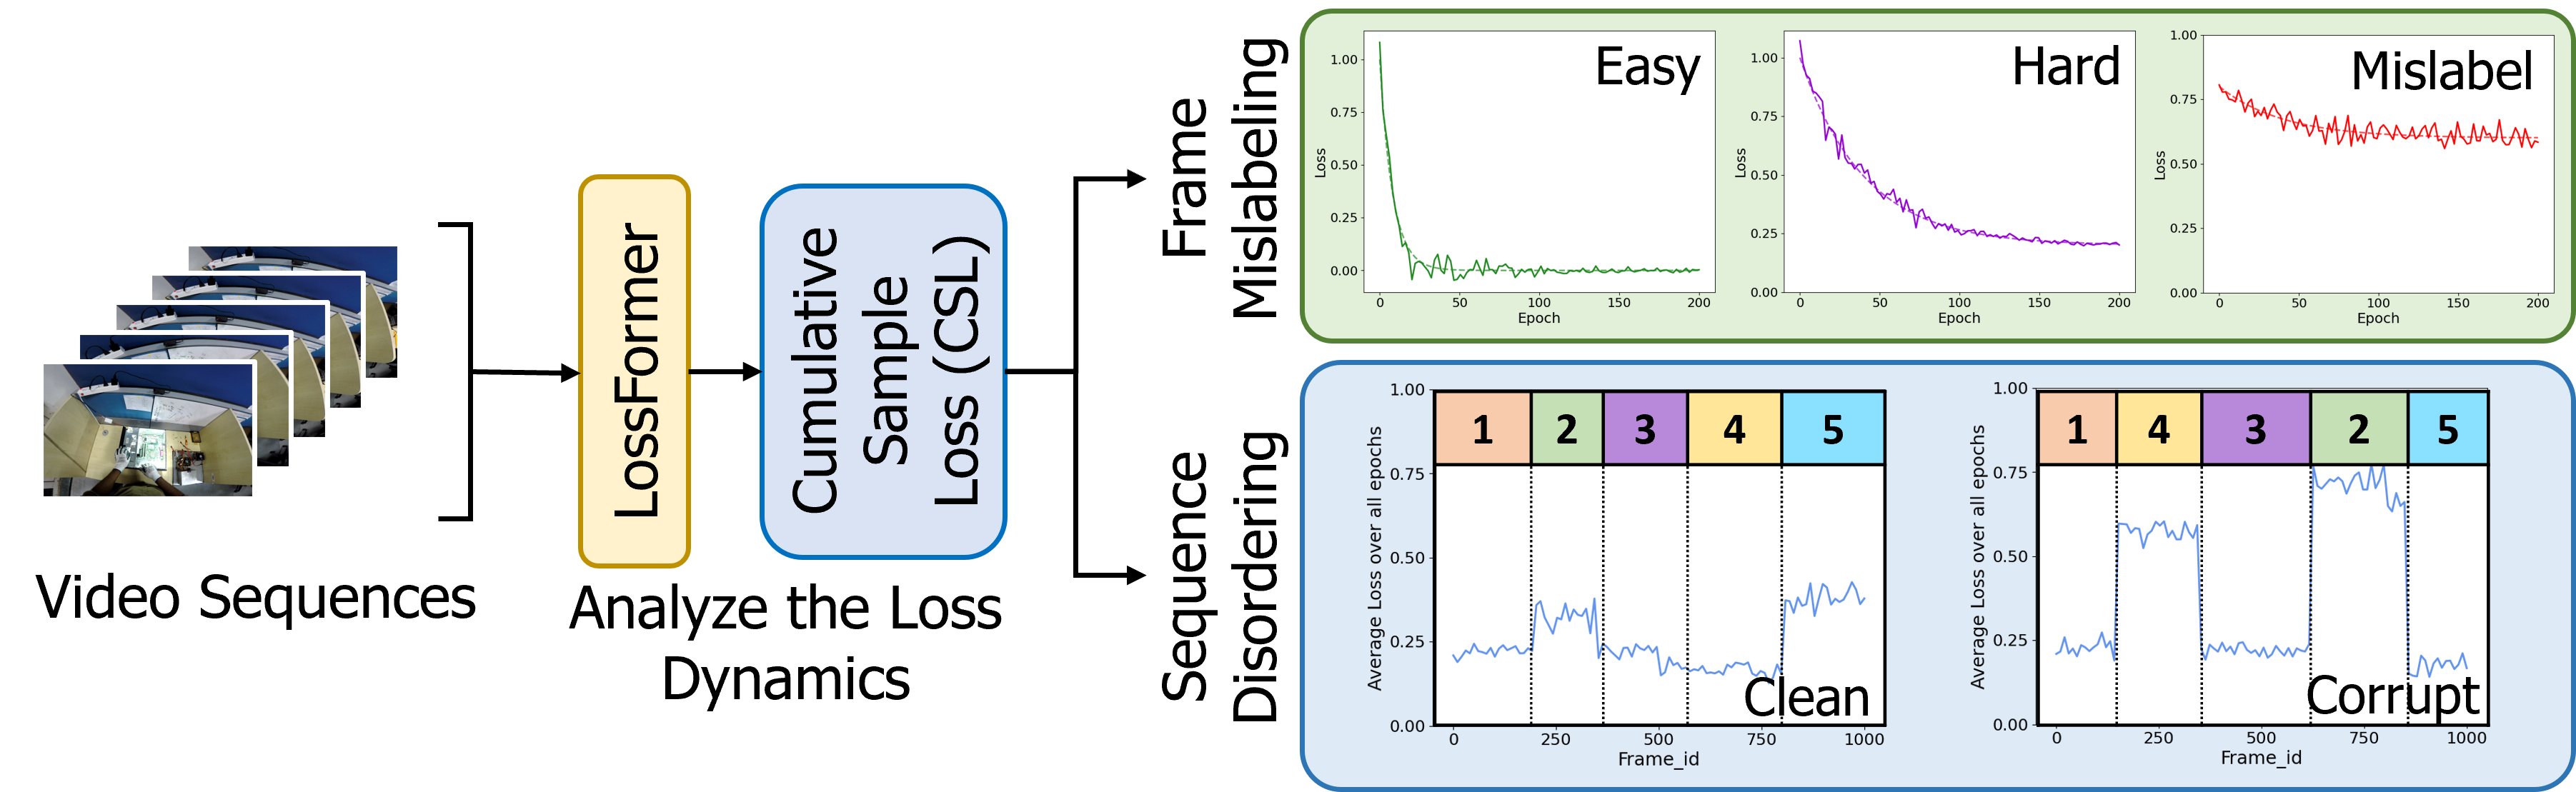
\includegraphics[width=0.85\linewidth]{Figures/Figure1.png}
    \caption{Overview of our CSL-based framework for detecting annotation errors in video datasets. Top right: Frames with correct labels exhibit low and stable sample losses (Easy), while mislabeled or ambiguous frames (Hard, Mislabel) maintain high or erratic loss trajectories. Bottom right: Sequence-level CSL reveals phase disordering-correctly labeled sequences show smooth loss trends aligned with phase boundaries, whereas corrupted sequences exhibit temporal inconsistencies and abrupt transitions in loss curves.}
    \label{fig:enter-label}
    \vspace{-1em}
\end{figure*}

Recent efforts to address corrupted data have explored corrective machine unlearning \cite{goel2024corrective}, which aims to retrospectively `forget' the influence of harmful samples from trained models. However, most unlearning methods assume prior knowledge of which samples are corrupted, enabling a binary separation into \textit{retain} and \textit{forget} sets. In practice, accurately identifying mislabeled or temporally disordered samples remains an open problem \cite{garg2023memorization}. This challenge is amplified in video datasets, where each sample consists of long sequences with dense frame-level annotations, making error localization substantially more difficult than in static image data.

To address this gap, we propose a novel lightweight, model-agnostic framework for automatically detecting annotation errors in temporally labeled video datasets by analyzing loss dynamics. Our approach is based on the \textbf{Cumulative Sample Loss (CSL)}, which measures how persistently difficult each frame is to learn across training epochs. By evaluating frame-level loss trajectories over saved training checkpoints, CSL serves as a proxy for annotation reliability ~\cite{dataset_cartography, deepak_angularloss, loss_importance}. Frames affected by semantic mislabeling or temporal disordering tend to maintain consistently high loss, whereas correctly labeled frames typically converge early.
Our method requires no access to ground-truth noise patterns, no additional supervision, and no retraining. Beyond identifying isolated mislabeled frames, CSL also exposes sequence-level temporal inconsistencies, which manifest as sharp loss fluctuations around phase boundaries. As illustrated in Figure~\ref{fig:enter-label}, this enables unified detection of both semantic and temporal annotation errors.
We evaluate our approach on two temporally structured video benchmarks, Cholec80 and EgoPER, spanning surgical workflow analysis and egocentric procedural understanding. On EgoPER, our method achieves frame-level AUC improvements of up to \textbf{4.6 points} over prior state-of-the-art methods and consistently exceeds \textbf{59\%} segment-level error detection accuracy across all tasks. On Cholec80, our framework reliably localizes both injected mislabeling and phase disordering without prior knowledge of corruption locations.

Our contributions are as follows:
\vspace{-1em}
\begin{itemize} [leftmargin=*]
    \item We introduce a model-agnostic and training-free framework for detecting annotation errors in temporally labeled video datasets using cumulative sample loss.
    
    \vspace{-2mm}
    \item We show that loss trajectories naturally distinguish clean labels from both semantic mislabeling and temporal disordering without requiring noise annotations or additional supervision.

    \vspace{-2mm}
    \item We demonstrate state-of-the-art performance on EgoPER and strong results on Cholec80, outperforming existing video anomaly and error detection baselines.
\end{itemize}

%%%%%%%%%%%%%%%%%%% Related Works
\vspace{-1em}
\section{Related Work}
\vspace{-0.2em}
\paragraph{Label Noise and Error Detection:}
Recent studies have revealed that label errors are more prevalent in benchmark datasets. For example, \cite{athalye} reported that approximately 6\% of labels in the ImageNet validation set are incorrect, while 3--4\% of samples across widely used vision, NLP, and audio datasets contain erroneous annotations. Early work on noisy supervision primarily modeled label noise as random corruption and focused on robust loss functions. However, real-world annotation errors are often systematic and structured, motivating methods that explicitly identify mislabeled samples \cite{label_errors_learning_1}.

Traditional label-cleaning methods draw on various heuristics to flag potential mislabels. Deep networks tend to learn correctly labeled samples faster than noisy ones, making \textit{loss dynamics} a useful signal for error detection. Samples that consistently exhibit high loss or unstable predictions across epochs are often flagged as mislabeled \cite{label_errors_learning_2}. Additional approaches monitor classifier disagreement during cross-validation or detect outliers in feature space \cite{chen2019understanding}. Ensemble-based methods such as \textit{Confident Learning} \cite{northcutt} identify label issues based on prediction agreement, while \textit{influence functions} trace the impact of individual samples on model predictions to uncover mislabeled data \cite{label_errors_learning_3}.

\vspace{-0.6em}
\paragraph{Self-Correction and Unsupervised Approaches:}
Beyond explicit error detection, several methods aim to mitigate label noise through self-correction. Unsupervised techniques leverage embedding-space clustering and nearest-neighbor analysis to identify anomalous labels \cite{Li_2021_ICCV}. Self-training and bootstrapping methods use model confidence or pseudo-labels to iteratively refine annotations \cite{label_errors_learning_4,label_errors_learning_6,label_errors_learning_7}. Other approaches incorporate noise-aware layers or auxiliary modules to explicitly model label corruption during training \cite{label_errors_learning_5}. While effective in static datasets, these methods often assume independent samples and struggle to capture temporal dependencies inherent to video data.

\vspace{-0.6em}
\paragraph{Noisy Supervision and Unlearning in Video:}
Handling noisy labels in video presents unique challenges due to temporal correlations and structured label dependencies. In addition to semantic mislabeling, video datasets frequently suffer from temporal misalignment and disordering, where labels are assigned to incorrect time segments. Prior work has explored \textit{relaxed} loss formulations for temporal event detection to reduce sensitivity to timestamp inaccuracies \cite{label_errors_learning_3}, as well as adaptations of co-teaching strategies for sequential data. However, as noted by \cite{label_errors_learning_10}, direct extensions of image-based noise-robust learning methods often fail in video settings due to temporal complexity and multi-modal cues.

More recently, machine unlearning has emerged as a promising direction for mitigating the impact of corrupted data \cite{kodge2025sap, goel2024corrective, kurmanji2023towards}. These methods aim to remove the influence of harmful samples from trained models but typically rely on prior knowledge of which samples are corrupted. In temporally labeled video datasets, accurately identifying such samples remains a largely unsolved problem. Our work directly addresses this gap by proposing a unified, training-free framework for detecting both semantic and temporal annotation errors using loss dynamics.


%%%%%%%%%%%%%%%%%%% Methodology
\begin{figure*}[!ht]
    \centering
    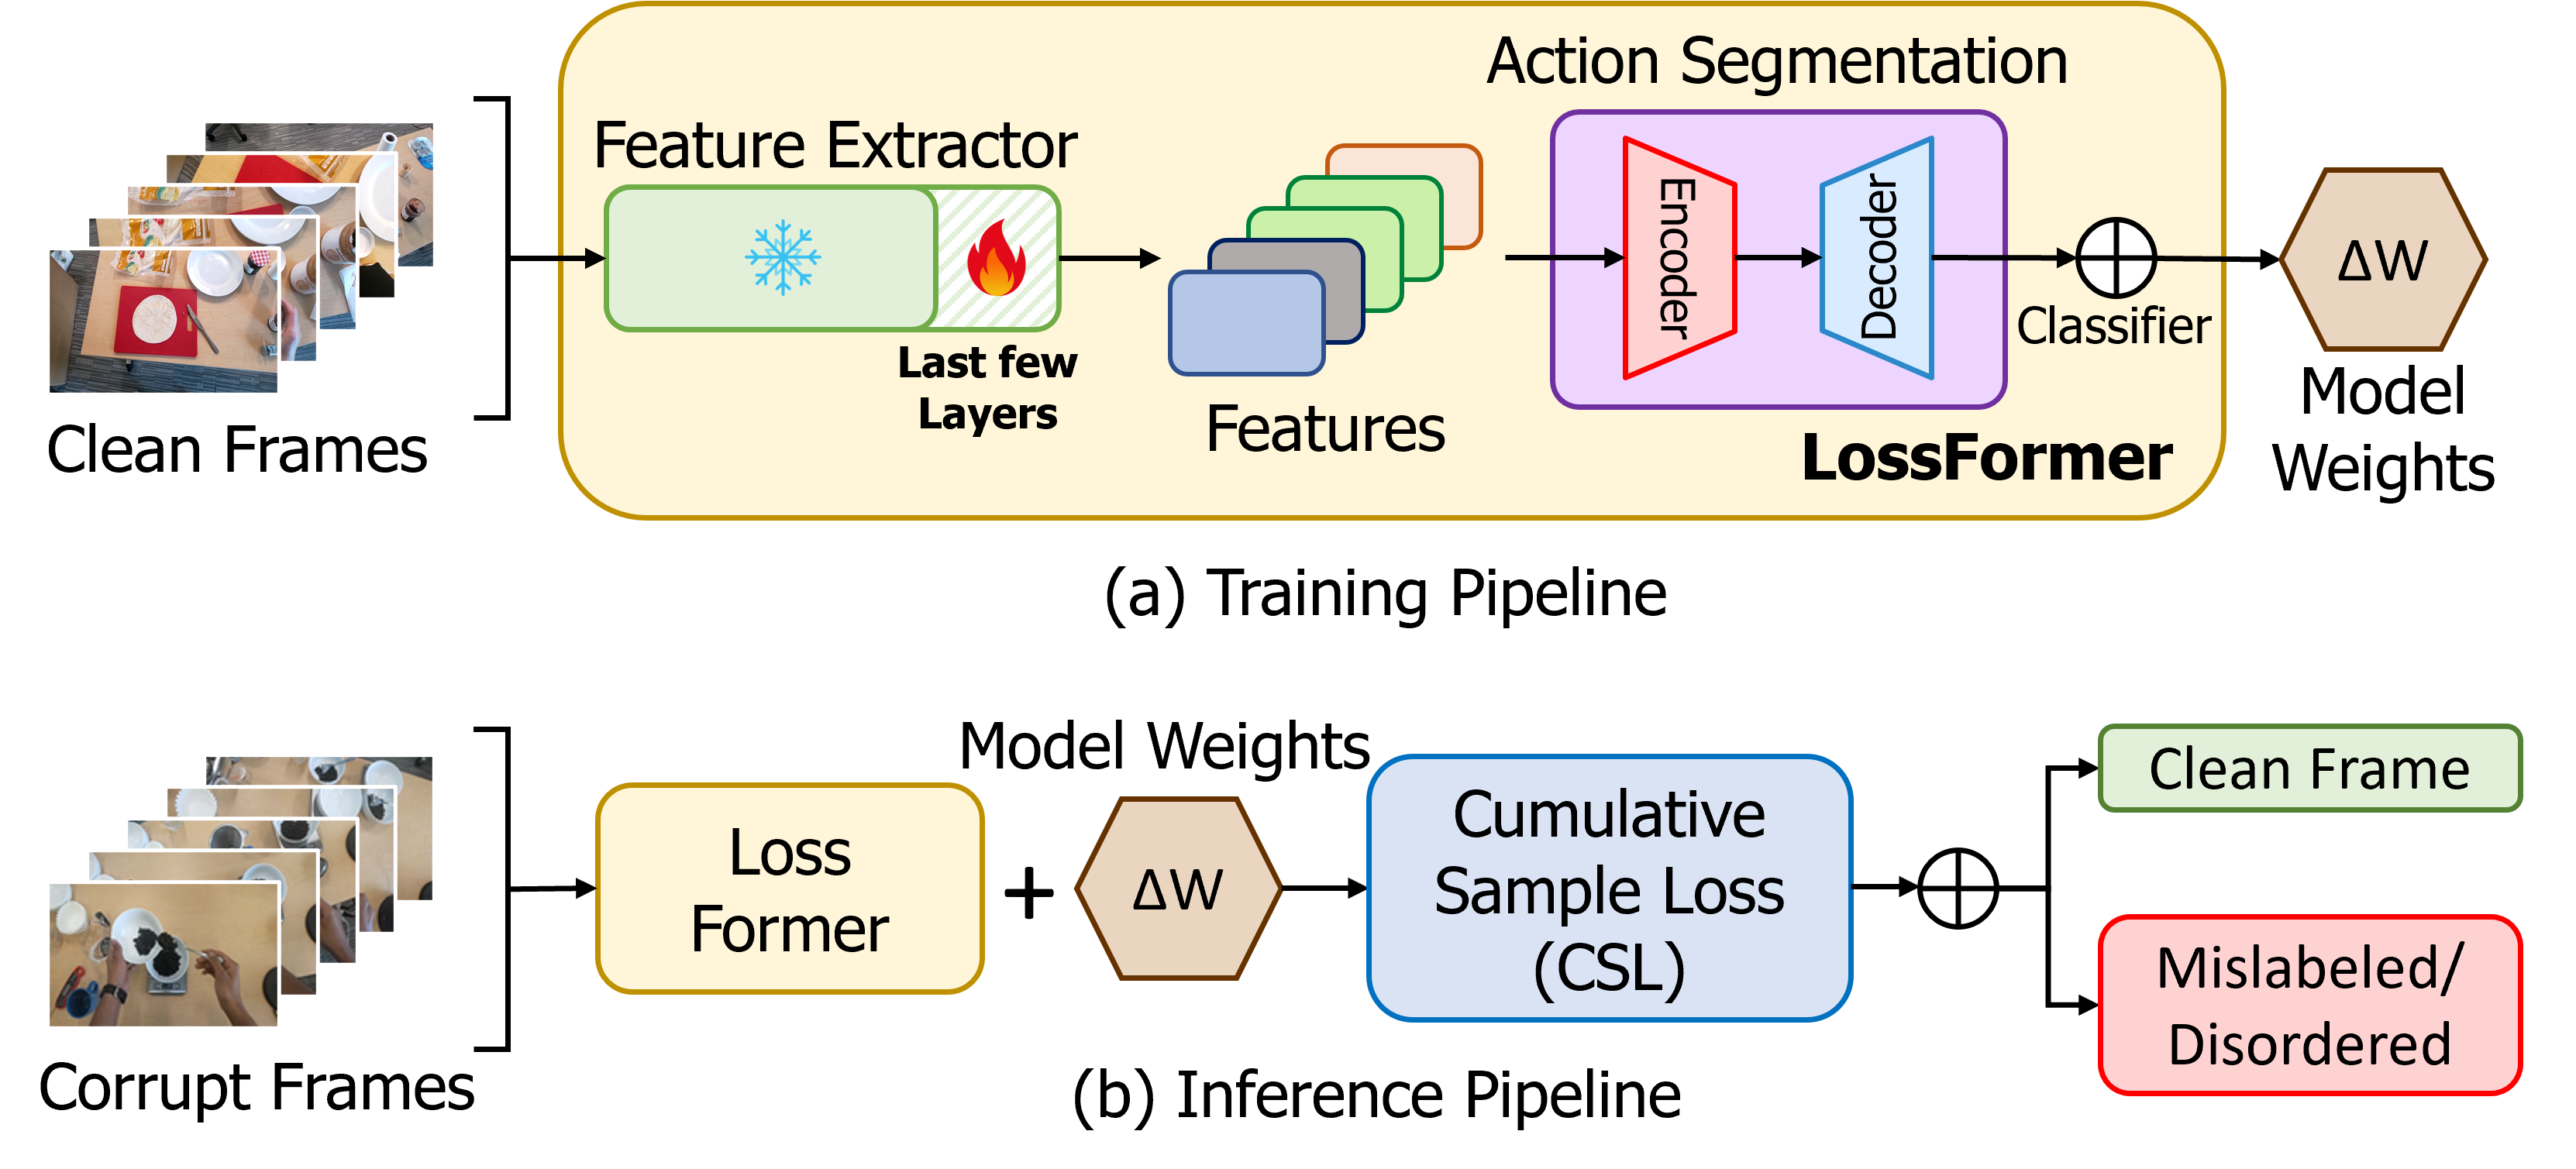
\includegraphics[width=0.8\linewidth]{Figures/Figure2.png}
    \vspace{-0.4em}
    \caption{(a) Training: A ResNet-18 Feature Extractor (FE) extracts frame features, which are passed through the ViT-B/16-based LossFormer for action segmentation. (b) Inference: CSL is computed from per-frame loss over training epochs and used to detect mislabeled or disordered frames.}
    \label{fig:pipeline}
    \vspace{-1em}
\end{figure*}

\vspace{-0.4em}
\section{Methodology}
\vspace{-0.4em}
\label{sec:method}
We propose a lightweight, model-agnostic framework for detecting annotation errors in temporally labeled video datasets using \textbf{loss dynamics}. Our key idea is simple: if a frame is correctly labeled, models typically learn it early and its loss drops quickly; if a frame is mislabeled or temporally inconsistent, the model struggles to fit it and its loss remains persistently high (or unstable) across training. We capture this behavior by computing the \textbf{Cumulative Sample Loss (CSL)} from per-frame loss trajectories evaluated over saved training checkpoints. CSL score serves as a proxy for \textit{memorization} \cite{ravikumar2025towards}, enabling us to flag mislabeled frames and temporally inconsistent sequences-without the need for retraining or prior access to label noise distributions.

\vspace{-0.6em}
\paragraph{Problem Setup:}
Let $\mathcal{D}=\{(X^{(i)},Y^{(i)})\}_{i=1}^{N}$ be a dataset of $N$ videos. Each video
$X^{(i)}=\{x^{(i)}_t\}_{t=1}^{T_i}$ contains $T_i$ frames, and
$Y^{(i)}=\{y^{(i)}_t\}_{t=1}^{T_i}$ are frame-level labels with $y^{(i)}_t \in \mathcal{Y}$.
Our goal is to identify frames whose annotations are unreliable due to:
(i) \textit{semantic mislabeling} (incorrect class/phase), and/or
(ii) \textit{temporal disordering} (labels are correct locally but violate the expected order).
We do \emph{not} assume access to ground-truth corruption masks, noise rates, or extra supervision.

\vspace{-0.6em}
\paragraph{Overview of the Two-Stage Framework:}
\vspace{-0.5em}
Our framework has two stages:
\vspace{-0.5em}
\begin{enumerate}[leftmargin=*]
    \item \textbf{Training with checkpointing:} Train any temporal video model normally for $E$ epochs and save model checkpoints $\{\theta^{(1)},\dots,\theta^{(E)}\}$.
    \vspace{-0.5em}
    \item \textbf{Post-hoc auditing:} For each test (or audit) video, run inference using every checkpoint to compute a \emph{loss trajectory} per frame. Aggregate this trajectory to obtain CSL scores, then flag high-CSL frames (and optionally segments) as potential annotation errors.
\end{enumerate}
\vspace{-1em}
This design is \textbf{training-free at audit time}: once checkpoints exist, detection requires no retraining, fine-tuning, or extra models.

\vspace{-0.4em}
\subsection{Model Architecture}
\label{subsec:architecture}
Although our method is model-agnostic, we instantiate it using a two-stage architecture (Figure~\ref{fig:pipeline}):

\vspace{-0.4em}
\paragraph{Feature Extractor:}
We use a ResNet-18 backbone pretrained on ImageNet21K~\cite{image_net} to extract per-frame features. Given a frame $x_t$,
\vspace{-0.4em}
\begin{equation}
\mathbf{h}_t = f_{\text{ResNet18}}(x_t), \quad \mathbf{h}_t \in \mathbb{R}^{512}.
\vspace{-0.4em}
\end{equation}
We freeze early layers to preserve generic visual representations and fine-tune the final layers for domain adaptation.

\vspace{-0.4em}
\paragraph{Temporal Segmentation Backbone.}
Frame features are passed to a Transformer-based temporal model (e.g., LossFormer, a temporal segmentation backbone based on the ViT-B/16 architecture~\cite{attention}), to produce contextualized features:
\vspace{-0.4em}
\begin{equation}
\mathbf{h}'_t = f_{\text{Transformer}}(\mathbf{h}_{1:T})_t.
\vspace{-0.4em}
\end{equation}

\vspace{-0.4em}
\paragraph{Classifier Head.}
We map $\mathbf{h}'_t$ to label probabilities with a lightweight MLP head:
\vspace{-0.4em}
\begin{align}
\mathbf{z}_t &= W_3\Big(\sigma(\mathrm{LN}(W_2\,\sigma(\mathrm{LN}(W_1\mathbf{h}'_t + b_1)) + b_2))\Big) + b_3, \notag\\
\hat{\mathbf{y}}_t &= \mathrm{softmax}(\mathbf{z}_t),
\vspace{-0.4em}
\end{align}
with $W_1 \in \mathbb{R}^{128 \times 512}$, $W_2 \in \mathbb{R}^{32 \times 128}$, $W_3 \in \mathbb{R}^{|\mathcal{Y}| \times 32}$, $\sigma(\cdot)$ as ReLU activation, and LN denotes LayerNorm. Dropout layers (with 0.5 and 0.3 rates) are applied between layers to prevent overfitting.

\subsection{Training Objective and Checkpoint Saving}
We train for the model for $E$ epochs and preserve the model checkpoints ($\{\theta^{(1)}, \theta^{(2)}, \dots, \theta^{(E)}\}$) at each training epoch. To handle class imbalance, we use class-weighted cross-entropy. For frame $x_t$ at epoch $e$, the loss is computed as:
\vspace{-0.4em}
\begin{equation}
\ell^{(e)}_t = -\sum_{c=1}^{|\mathcal{Y}|}\alpha_c\,\mathbb{1}[y_t=c]\log {p}^{(e)}_{t,c},
\vspace{-0.4em}
\end{equation}
where $p_{t,c}^{(e)}$ is the predicted probability for class $c$ at epoch $e$ and $y_{t,c}$ is a binary indicator (0 or 1) indicating whether the true label is class $c$. $\alpha_c$ denotes the class-specific weight and is inversely proportional to the frequency of class $c$ in the training set.

\vspace{-0.4em}
\subsection{Loss Trajectories and Cumulative Sample Loss}
\label{subsec:csl}
After training, we compute per-frame \textbf{loss trajectories} by evaluating each frame using every saved checkpoint. For a frame $x_t$ with annotation $y_t$, we compute the loss across each saved checkpoint $\theta^{(e)}$:
\vspace{-0.4em}
\begin{equation}
\hat{\ell}^{(e)}_t = \mathcal{L}\big(f_{\theta^{(e)}}(x_t),\, y_t\big), \quad e=\{1,\dots,E\}.
\vspace{-0.4em}
\end{equation}
We then define the average \textbf{Cumulative Sample Loss (CSL)} for each frame $x_t$ as the average loss over the full training trajectory:
\vspace{-0.4em}
\begin{equation}
\mathrm{CSL}(x_t) = \frac{1}{E}\sum_{e=1}^{E}\hat{\ell}^{(e)}_t.
\vspace{-0.4em}
\end{equation}
Correctly labeled frames tend to become ``easy'' early. As training progresses, the model quickly assigns high probability to the correct label, and $\hat{\ell}^{(e)}_t$ decreases. In contrast, frames with consistently high CSL values indicate the difficulty of the model to confidently associate them with their annotated labels throughout the model checkpoints, signifying potential annotation errors such as mislabeling or temporal disordering.

\paragraph{Smoothing and Sequence-Level Signals:}
Raw CSL values can be noisy due to local visual ambiguity or boundary transitions. To better localize error regions, we optionally compute a temporally smoothed CSL curve within each video:
\vspace{-0.4em}
\begin{equation}
\widetilde{\mathrm{CSL}}(t) = \frac{1}{2w+1}\sum_{j=-w}^{w} \mathrm{CSL}(x_{t+j}),
\vspace{-0.4em}
\end{equation}
where $w$ is a small window size. In practice, smoothing helps reveal temporally coherent error segments: semantic mislabeling often yields sustained high CSL over a contiguous region, while disordering frequently produces sharp spikes around phase transitions.

\vspace{-0.4em}
\subsection{Anomaly Scoring and Error Flagging}
We treat both mislabeling and disordering as annotation errors and flag frames using a threshold or percentile rule.

\vspace{-0.4em}
\paragraph{Threshold-based detection:}
We compute a threshold $\tau$ based on the CSL distribution from a validation set (or from robust statistics over the video) and mark frames as anomalous:
\vspace{-0.4em}
\begin{equation}
\mathrm{Anomaly}(x_t)=
\begin{cases}
1, & \text{if } \widetilde{\mathrm{CSL}}(t) > \tau, \\
0, & \text{otherwise.}
\end{cases}
\vspace{-0.8em}
\end{equation}

\vspace{-0.4em}
\paragraph{Percentile-based detection:}
When tuning $\tau$ is undesirable, we rank frames by $\widetilde{\mathrm{CSL}}(t)$ and flag the top-$k\%$ as candidates. This is convenient for dataset auditing when the goal is to surface the most suspicious regions for review.

Correctly labeled frames typically experience a rapid loss decline during training, whereas frames affected by annotation errors-whether due to semantic mislabeling or temporal inconsistencies-retain high loss, signaling discordance with the learned representation. Interestingly, in mislabeling cases, nearly the entire segment often accumulates high CSL due to persistent semantic disagreement (Figure~\ref{fig:csl_maps}). In contrast, disordering errors tend to localize around transition phases, where the model, despite memorization of the overall task structure, encounters temporal inconsistencies that manifest as sharp CSL spikes.

\vspace{-0.4em}
\subsection{Complexity and Practicality}
Let $T$ be the number of frames in a video and $E$ be the number of saved checkpoints. Auditing requires $E$ forward passes per frame (or one forward pass per checkpoint over the full video sequence), resulting in $O(E\cdot T)$ inference cost. Importantly, this cost is \emph{embarrassingly parallel} over checkpoints and videos and requires no gradient computation, making it efficient on modern accelerators.

%%%%%%%%%%%%%%%%%%% Algorithm
\vspace{-0.4em}
\subsection{Algorithm}
\begin{algorithm}[H]
\caption{Annotation Error Detection via CSL}
\label{alg:csl_framework}
\textbf{Inputs:} Training dataset $\mathcal{D}_{train}$, test dataset $\mathcal{D}_{test}$, model $f_{\theta}$, epochs $E$, CSL threshold $\tau$.

\textbf{Output:} Frame-wise anomaly predictions for $\mathcal{D}_{test}$.

\begin{algorithmic}[1]
\STATE Initialize model $f_{\theta^{(0)}}$ (any temporal backbone, e.g: ResNet-18).
\FOR{epoch $e = 1, 2, \dots, E$}
    \STATE Train $f_{\theta^{(e)}}$ using weighted cross-entropy loss on dataset $\mathcal{D}_{train}$.
    \STATE Save model checkpoint $\theta^{(e)}$.
\ENDFOR

\FOR{video $(X,Y)\in \mathcal{D}_{\text{test}}$}
    \FOR{frame $x_t \in X$}
        \STATE Initialize cumulative loss: $ \text{CSL}(x_t) = 0 $
        \FOR{epoch $e = 1, 2, \dots, E$}
            \STATE Compute frame-level loss trajectory: $\hat{\ell}_t^{(e)} = \mathcal{L}(f_{\theta^{(e)}}(x_t), y_t)$
            \STATE Update CSL: $\text{CSL}(x_t) \leftarrow \frac{1}{E}\sum_{e=1}^{E}\hat{\ell}^{(e)}_t$.
        \ENDFOR
    \ENDFOR
    \STATE Flag errors using threshold $\tau$ or top-$k\%$ ranking.
    \[ \text{Anomaly}(x_t) = \begin{cases} 1, & \text{if CSL}(x_t) > \tau \\ 0, & \text{otherwise} \end{cases} \]
\ENDFOR
\end{algorithmic}
\end{algorithm}

%%%%%%%%%%%%%%%%%%% Results
\vspace{-0.8em}
\section{Experiments and Results}
We evaluate the effectiveness of our CSL-based annotation error detection framework on two temporally structured video datasets from distinct domains: a surgical workflow dataset (Cholec80) and an egocentric procedural dataset (EgoPER). Our evaluation focuses on detecting both semantic mislabeling and temporal disordering under controlled annotation corruptions.

\vspace{-0.4em}
\subsection{Dataset}
\textbf{Cholec80}~\cite{surgical_endonet} is a surgical workflow dataset comprising 80 laparoscopic cholecystectomy videos, each annotated at the frame level across seven distinct surgical phases. Following the standard protocol, we use 50 videos for training, 10 for validation, and 20 for testing. Videos are sampled at 15 fps and resized to $224 \times 224$.
To evaluate robustness to annotation errors, we introduce two types of synthetic corruption in the test set:
\begin{itemize}
    \vspace{-0.8em}
    \item \textbf{Mislabeling:} Continuous frame segments in 10 test videos are assigned incorrect phase labels, simulating realistic semantic annotation mistakes.
    \vspace{-0.4em}
    \item \textbf{Temporal Disordering:} In another 10 test videos, two contiguous phases are swapped while preserving frame-level labels, resulting in correct semantics but incorrect temporal order.
\end{itemize}
\vspace{-0.4em}
These settings produce two separate evaluation splits, allowing isolated analysis of mislabeling and disordering.

\textbf{EgoPER.}~\cite{EgoPER} is a large-scale egocentric dataset containing over 28 hours of instructional videos captured with a head-mounted GoPro, curated for procedural task understanding and error detection. It spans five procedural tasks: preparing \textit{coffee}, making \textit{tea}, assembling a \textit{pinwheel} sandwich, cooking a \textit{quesadilla}, and making \textit{oatmeal}. Each video is annotated with fine-grained procedural steps and ground-truth transcripts indicating both correct and erroneous executions.

%%%%%%%%%%%%%%%%%%%%%%%%%%%%%%%%%%%%%%%%%%% Dataset table
\begin{table}[!ht]
\centering
\caption{Statistics of datasets used. The test sets contain corrupted annotations such as label noise and step disorder.}
\label{tab:dataset}
\resizebox{\linewidth}{!}{%
\begin{tabular}{lccc}
\toprule[1.5pt]
\textbf{Dataset / Task} & \textbf{Train / Test} & \textbf{Duration (min)} & \textbf{Actions} \\
\midrule[1pt]
\multicolumn{4}{l}{\textbf{Cholec80}} \\
\hspace{0.5em}Full Dataset & 60 / 10+10 & 38.0 / 32.3 & 7 \\
\midrule
\multicolumn{4}{l}{\textbf{EgoPER}} \\
\hspace{0.5em}Coffee     & 32 / 35 & 8.4 / 9.3 & 15 \\
\hspace{0.5em}Pinwheels  & 42 / 42 & 5.6 / 4.2 & 13 \\
\hspace{0.5em}Tea        & 47 / 32 & 2.6 / 2.5 & 10 \\
\hspace{0.5em}Quesadilla & 48 / 32 & 1.6 / 1.8 & 8 \\
\hspace{0.5em}Oatmeal    & 44 / 32 & 4.2 / 4.3 & 11 \\
\bottomrule[1.5pt]
\end{tabular}%
}
\end{table}

For our experiments, we derive frame-level phase labels and simulate additional annotation noise, including step reordering, label duplication, and insertion of incorrect steps. These corruptions reflect common inconsistencies in real-world instructional datasets. Across both datasets in Table~\ref{tab:dataset}, timestamps are normalized and videos are trimmed to align cleanly with phase boundaries to ensure consistent per-frame supervision.This preprocessing allows consistent per-frame supervision and alignment with LossFormer's temporal modeling capabilities.

%%%%%%%%%%%%%%%%%%%%%%%%%%%%%%%%%%%%%%%%%%% Mislabeling graph figure
\begin{figure*}[!ht]
    \centering
    
\includegraphics[width=0.9\linewidth]{Figures/Figure3.png}
    \caption{Qualitative results of error detection on EgoPER and Cholec80. The top row shows representative frames, while the bottom row shows the cumulative sample loss trajectory across time. Our method accurately identifies corrupted regions (red spikes) using a task-specific threshold $\tau$.}
    \label{fig:error_detection_traj}
    \vspace{-1em}
\end{figure*}

\subsection{Evaluation Metrics}
\label{subsec:metrics}
We evaluate CSL-based annotation error detection using both segment-level and frame-level metrics.
\vspace{-0.8em}
\paragraph{Segment-wise Error Detection Accuracy (EDA):}
EDA measures the proportion of ground-truth erroneous segments successfully detected within the top-$k\%$ of frames ranked by the error score. A segment is considered detected if at least one of its frames is flagged.  We compute EDA as \( |\mathcal{D}_e \cap \text{GT}_e| / |\text{GT}_e| \), where, $\mathcal{D}_e$ and $\text{GT}_e$ denote the predicted and ground-truth erroneous segments.
\vspace{-0.6em}
\paragraph{Frame-wise Micro-AUC:}
We also compute the micro Area Under the ROC Curve (AUC) using frame-level error probabilities. AUC provides a threshold-independent measure of separability between clean and corrupted frames.

\vspace{-0.4em}
\subsection{Baselines}
\label{subsec:baselines}
We compare our method, \textbf{LossFormer}, against state-of-the-art video anomaly detection and procedural error detection methods adapted for annotation error detection. Baselines include HF$^2$-VAD~\cite{hf2vad} and its SSPCAB-enhanced variant~\cite{sspcab}, which rely on reconstruction and future-frame prediction, as well as S3R~\cite{s3r}, which synthesizes pseudo-anomalies using dictionary learning and learns a discriminative decision boundary. We also compare against EgoPED~\cite{EgoPER}, which combines action segmentation backbones (ActionFormer~\cite{ActionFormer}, MSTCN++~\cite{mstcn++}, DiffAct~\cite{diffact}) augmented with graph reasoning and hand-object interaction cues. A random baseline provides a lower bound. Unlike these methods, LossFormer detects annotation errors by modeling loss dynamics over training checkpoints rather than visual abnormality.

%%%%%%%%%%%%%%%%%%%%%%%%%%%%%%%%%%%%%%%%%%% Result table - EgoPER
\begin{table*}[!ht]
\centering
\caption{Performance comparison (EDA / AUC) on the \textbf{EgoPER} benchmark. LossFormer outperforms across all tasks in AUC and achieves competitive EDA, validating its ability to detect diverse annotation errors through cumulative loss dynamics.}
\label{tab:egoper_results}
\resizebox{\textwidth}{!}{%
\begin{tabular}{lcccccccccc}
\toprule[1.5pt]
\multirow{2}{*}{\textbf{Method}} &
\multicolumn{2}{c}{\textbf{Quesadilla}} &
\multicolumn{2}{c}{\textbf{Oatmeal}} &
\multicolumn{2}{c}{\textbf{Pinwheel}} &
\multicolumn{2}{c}{\textbf{Coffee}} &
\multicolumn{2}{c}{\textbf{Tea}} \\
\cmidrule(lr){2-3}\cmidrule(lr){4-5}\cmidrule(lr){6-7}\cmidrule(lr){8-9}\cmidrule(lr){10-11}
& \textbf{EDA} & \textbf{AUC}
& \textbf{EDA} & \textbf{AUC}
& \textbf{EDA} & \textbf{AUC}
& \textbf{EDA} & \textbf{AUC}
& \textbf{EDA} & \textbf{AUC} \\
\midrule[1pt]
Random                               & 19.9 & 50.0 & 11.8 & 50.0 & 15.7 & 50.0 &  8.2 & 50.0 & 17.0 & 50.0 \\
HF\textsuperscript{2}-VAD~\cite{hf2vad}            & 34.5 & 62.6 & 25.4 & 62.3 & 29.1 & 52.7 & 10.0 & 59.6 & 36.6 & 62.1 \\
HF\textsuperscript{2}-VAD + SSPCAB~\cite{sspcab}   & 30.4 & 60.9 & 25.3 & 61.9 & 33.9 & 51.7 & 10.0 & \textbf{60.1} & 35.4 & 63.2 \\
S3R~\cite{s3r}                                       & 52.6 & 51.8 & 47.8 & 61.6 & 50.5 & 52.4 & 16.3 & 51.0 & 47.8 & 57.9 \\
EgoPED (AF)~\cite{EgoPER}                            & 62.7 & 65.6 & 51.4 & 65.1 & \textbf{59.6} & 55.0 & 55.3 & 58.3 & 56.0 & 66.0 \\
\rowcolor[gray]{0.9}
\textbf{LossFormer (Ours)}                           & \textbf{63.1} & \textbf{68.2} & \textbf{55.4} & \textbf{67.1} & 50.9 & \textbf{57.3} & \textbf{55.8} & 59.6 & \textbf{59.9} & \textbf{70.2} \\
\bottomrule[1.5pt]
\end{tabular}%
}
\vspace{-1em}
\end{table*}

\vspace{-0.4em}
\subsection{Implementation Details}
\label{subsec:implementation}
LossFormer uses a ResNet-18 backbone for frame-level feature extraction and a ViT-B/16 Transformer for temporal modeling. Models are trained for 200 epochs using AdamW with a learning rate of $10^{-4}$ and class-weighted cross-entropy. Training takes approximately 12 hours on a single NVIDIA A100 GPU.
During inference, we compute the CSL for each frame by averaging loss values across all saved checkpoints. CSL signals are temporally smoothed, and frames are ranked to flag annotation errors using fixed percentile thresholds. All hyperparameters are selected via cross-validation. The framework is fully modular and does not require access to corrupted labels during training.

\vspace{-0.4em}
\subsection{Results}
\paragraph{EgoPER:}
\label{subsec:egoper_results}
Table~\ref{tab:egoper_results} reports segment-wise EDA and frame-wise AUC across five EgoPER tasks. LossFormer consistently achieves the highest AUC on all tasks, indicating strong frame-level discrimination between clean and corrupted annotations.
In particular, LossFormer reaches an AUC of \textbf{70.2} on \textit{Tea}, improving upon the strongest baseline EgoPED (66.0) by \textbf{6.4\%}, and an AUC of \textbf{68.2} on \textit{Quesadilla}, surpassing the best baseline by \textbf{2.6\%}. Averaged across all tasks, LossFormer improves AUC by \textbf{+3.2\%} while maintaining a strong average EDA of \textbf{57.0}.
Qualitative results in Figure~\ref{fig:error_visualization_egoper} show that LossFormer produces smoother and more temporally coherent predictions, significantly reducing false positives compared to frame-level anomaly detection methods such as HF$^2$-VAD.

\begin{figure}[!ht]
    \centering
    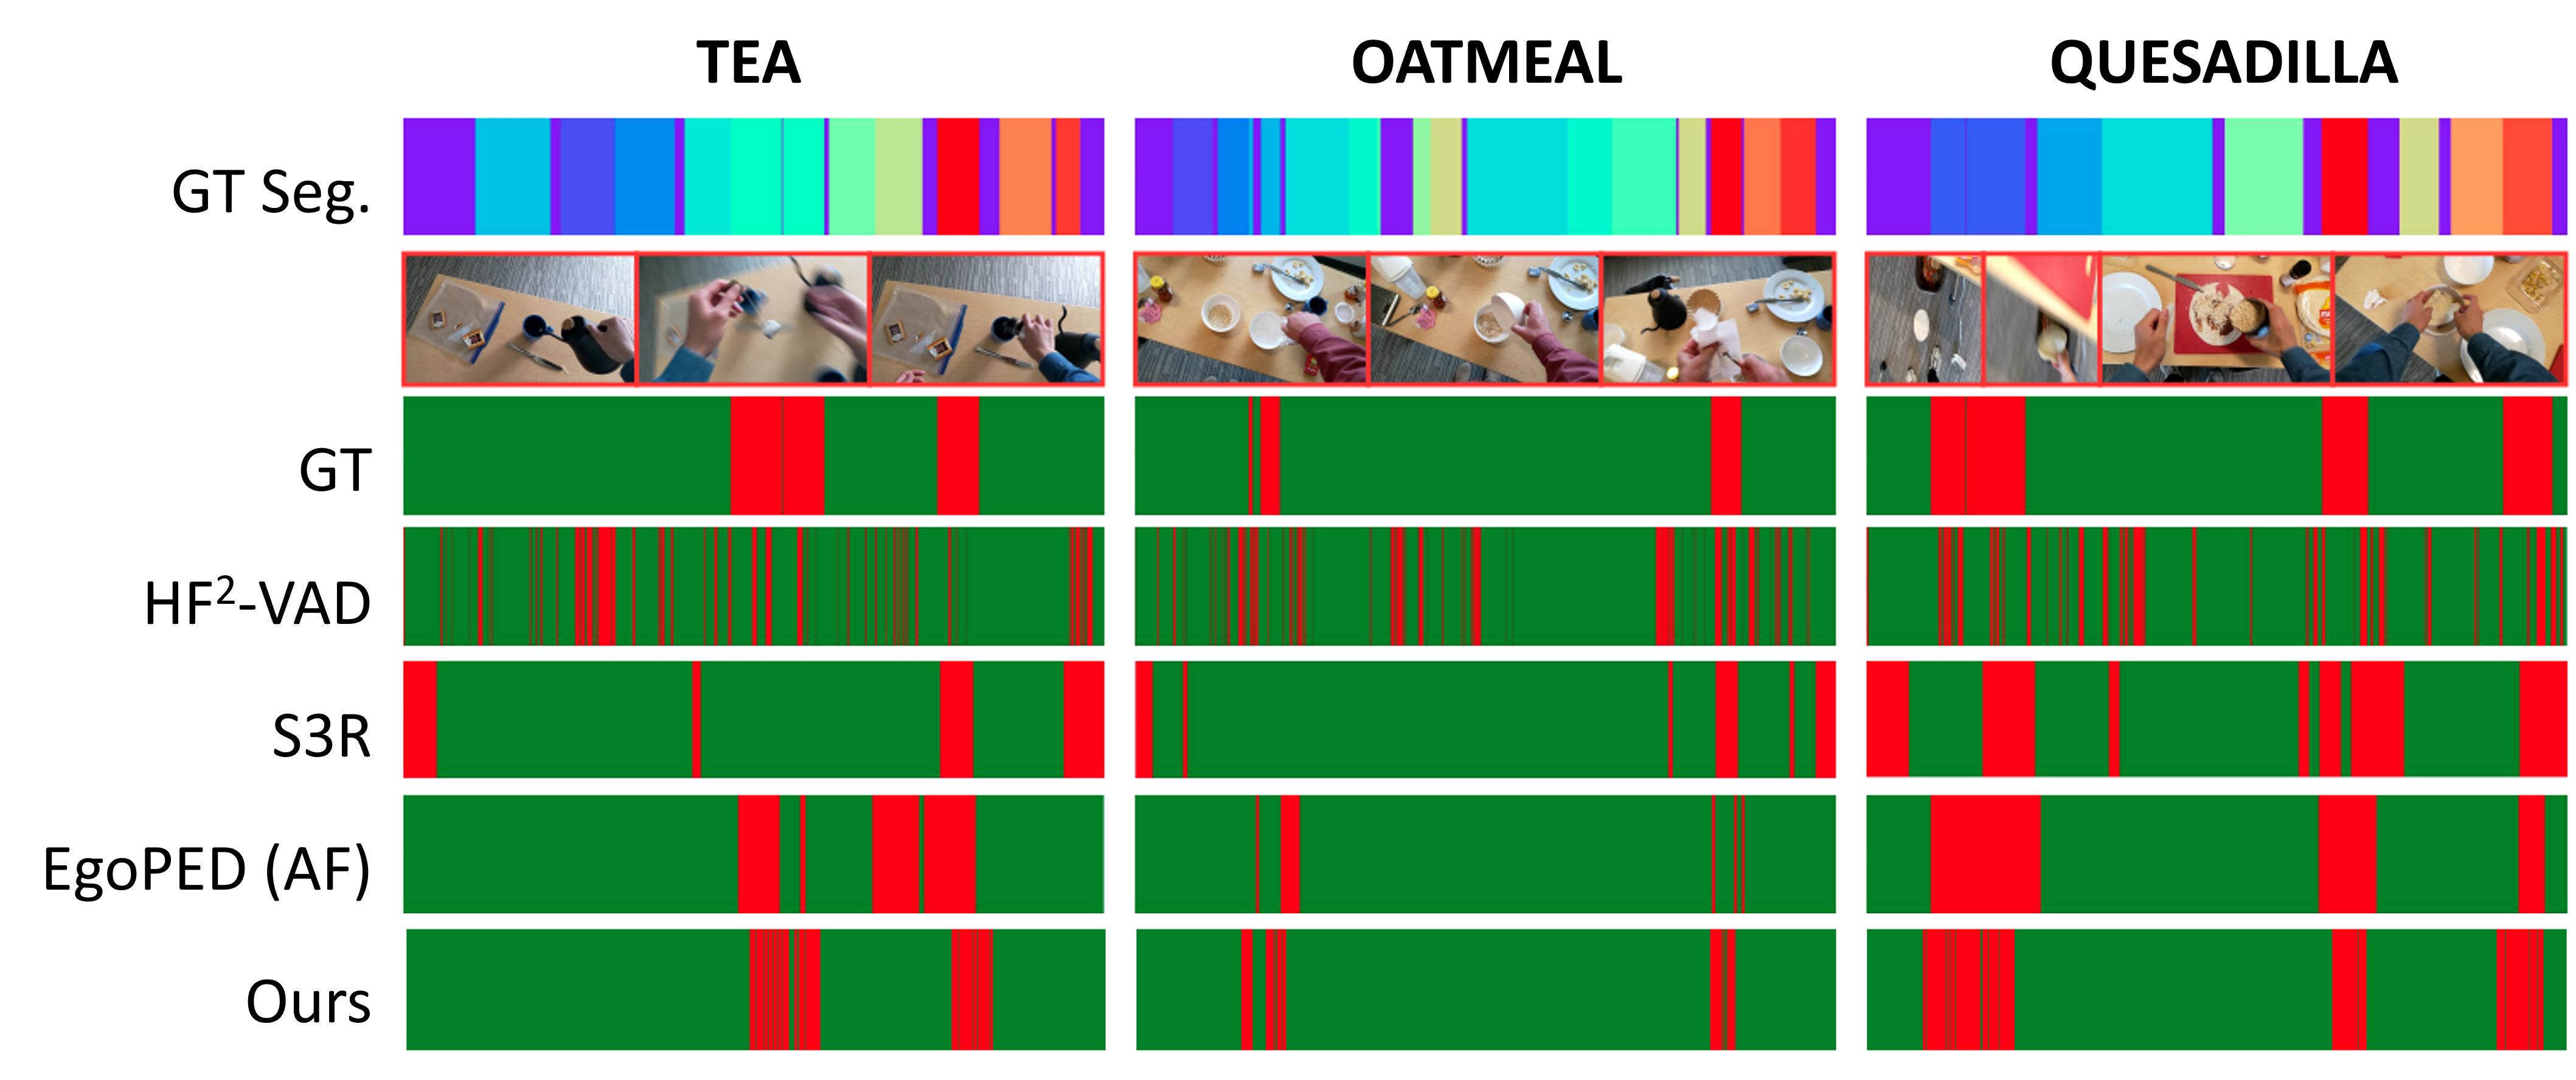
\includegraphics[width=\linewidth]{Figures/Figure4.png}
    \caption{Visualization of error detection across EgoPER dataset test sequences. Green indicates correct frames, red denotes detected annotation errors. Each row represents a different method, with our method (bottom row) shows precise localization of mislabelled or disordered segments.}
    \label{fig:error_visualization_egoper}
    \vspace{-1em}
\end{figure}

\vspace{-0.4em}
\paragraph{Cholec80:}
\label{subsec:cholec80_results}
We further evaluate generalization on the Cholec80 surgical dataset under both mislabeling and temporal disordering. Results are summarized in Table~\ref{tab:cholec80_results}. Under semantic mislabeling, LossFormer achieves an EDA of \textbf{85.9} and an AUC of \textbf{92.0}, outperforming the strongest baseline (EgoPED) by \textbf{+19.1\%} in EDA and \textbf{+20.7\%} in AUC. In the more challenging disordering scenario--where no prior baselines explicitly report results--LossFormer remains robust, achieving an EDA of \textbf{74.5} and an AUC of \textbf{78.5}. These results demonstrate LossFormer's unique ability to detect both semantic and temporal annotation errors in complex procedural workflows.

%%%%%%%%%%%%%%%%%%%%%%%%%%%%%%%%%%%%%%%%%%% Result table - Cholec80
\begin{table}[!ht]
\centering
\vspace{-0.2em}
\caption{Comparison of error detection performance (EDA / AUC) on the \textbf{Cholec80} dataset under two types of synthetic annotation errors: \textit{mislabeling} and \textit{temporal disordering}. LossFormer is the \textit{only method} evaluated on both error types, achieving state-of-the-art performance by a significant margin.}
\label{tab:cholec80_results}
\resizebox{\linewidth}{!}{%
\begin{tabular}{llcc}
\toprule[1.5pt]
\multicolumn{2}{c}{\textbf{Method}} & \textbf{EDA} & \textbf{AUC} \\
\midrule[1pt]
Random                             & --          & 24.1 & 50.0 \\
HF\textsuperscript{2}-VAD          & --          & 48.6 & 66.4 \\
HF\textsuperscript{2}-VAD + SSPCAB & --          & 50.3 & 68.1 \\
S3R                                & --          & 57.2 & 63.5 \\
EgoPED (AF)                        & --          & 66.8 & 71.2 \\
\midrule
\multirow{2}{*}{\textbf{LossFormer (Ours)}} 
& \cellcolor[gray]{0.9}\textbf{Mislabeled} 
& \cellcolor[gray]{0.9}\textbf{85.9} 
& \cellcolor[gray]{0.9}\textbf{92.0} \\
& \cellcolor[gray]{0.9}\textbf{Disordered} 
& \cellcolor[gray]{0.9}\textbf{74.5} 
& \cellcolor[gray]{0.9}\textbf{78.5} \\
\bottomrule[1.5pt]
\end{tabular}%
}
\vspace{-0.6em}
\end{table}

\vspace{-0.4em}
\subsection{Qualitative Analysis}
\label{subsec:qualitative}
Figure~\ref{fig:error_detection_traj} visualizes CSL trajectories for representative EgoPER and Cholec80 videos. Correctly labeled segments exhibit consistently low CSL, while mislabeled regions produce sustained spikes, and disordered segments show sharp peaks near phase transitions. Figure~\ref{fig:csl_maps} further illustrates these patterns across full sequences, highlighting how CSL naturally separates clean, mislabeled, and temporally inconsistent annotations. These patterns reinforce the effectiveness of our approach in capturing both spatial and temporal annotation inconsistencies through cumulative loss signals. Additional qualitative results are provided in the Supplementary Figure ~\ref{fig:csl_maps_ab}.

\begin{figure*}[!ht]
    \centering
    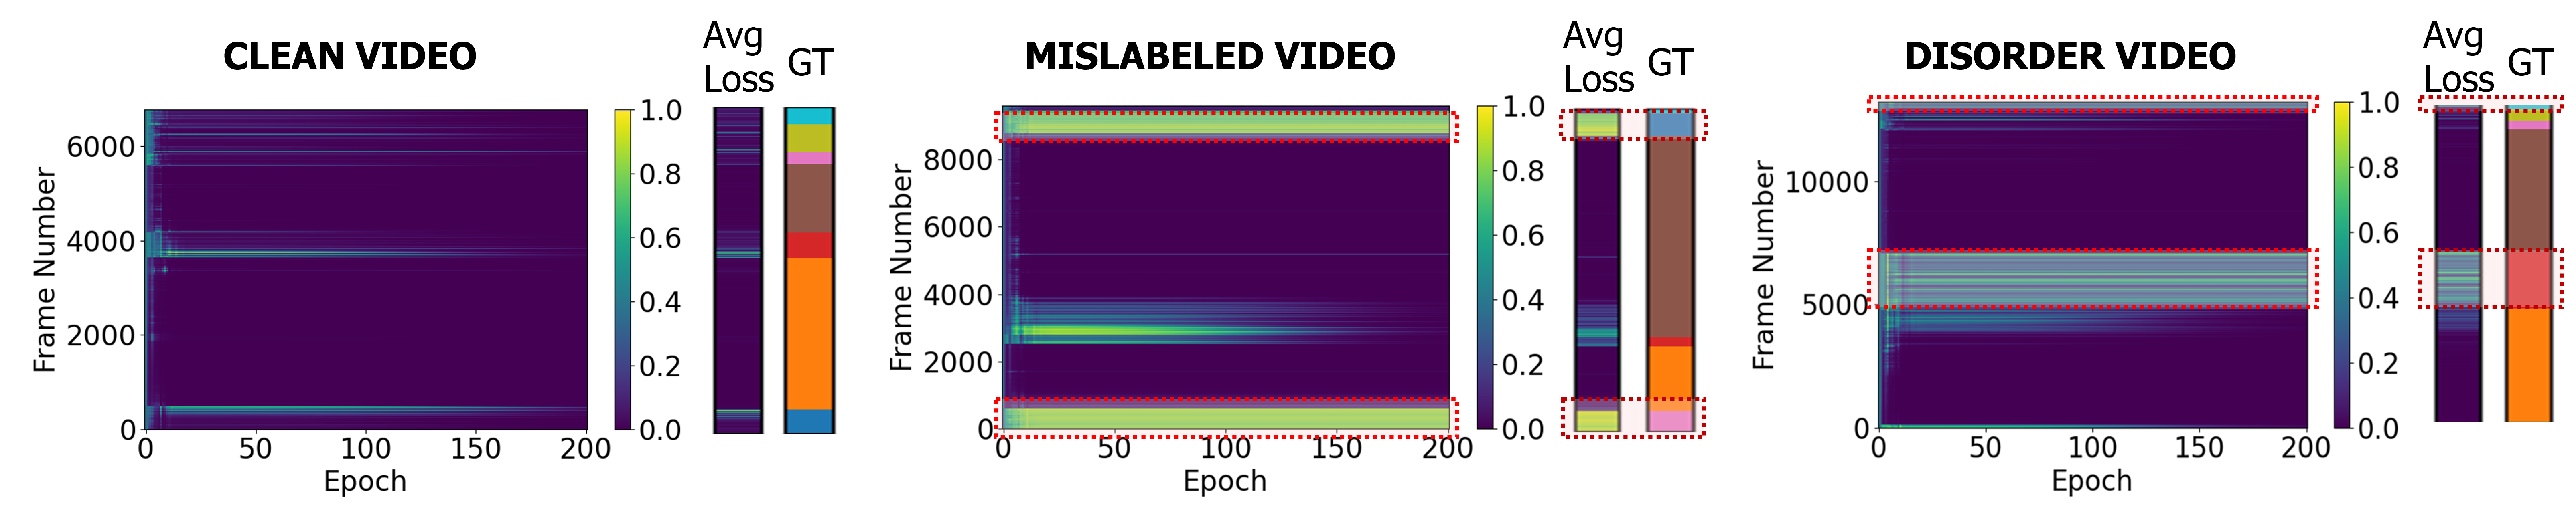
\includegraphics[width=0.9\linewidth]{Figures/Figure5.png}
    \caption{Visualization of Cumulative Sample Loss (CSL) trends across training epochs. Left: Correctly labeled data exhibits low CSL loss concentration. Center: Label misannotations correspond to high CSL spikes (red boxes). Right: Disordering induces high CSL activations, especially around phase transition boundaries.}
    \label{fig:csl_maps}
    \vspace{-1.4em}
\end{figure*}

\vspace{-0.4em}
\section{Ablation Studies}
\label{sec:ablation}
We conduct ablation studies to analyze which architectural and training choices most influence CSL-based annotation error detection. Our analysis focuses on three questions:
(i) how much domain adaptation is required in the feature extractor,
(ii) how temporal modeling capacity affects the detection of ordering errors, and
(iii) how robust the framework is when trained on noisy annotations.
All ablations are performed under controlled annotation corruption to isolate each factor.


%%%%%%%%%%%%%%%%%%%%%%%%%%%%%%%%%%%%%%%%%%% Ablation
\begin{table}[!ht]
\centering
\vspace{-0.5em}
\caption{AUC values of frozen and trainable ResNet18 across datasets.}
\label{tab:train_vs_frozen}
\begin{tabular}{llcc}
\toprule[1.5pt]
\multicolumn{2}{c}{\textbf{Dataset}} 
& \shortstack{\textbf{Frozen}\\\textbf{ResNet18}} 
& \shortstack{\textbf{Trainable}\\\textbf{ResNet18}} \\
\midrule[1pt]
Quesadilla & -- & 46.2 & 68.2 \\
Oatmeal    & -- & 41.4 & 67.1 \\
Pinwheel   & -- & 40.9 & 57.3 \\
Coffee     & -- & 36.7 & 59.6 \\
Tea        & -- & 48.1 & 70.2 \\
\midrule
\multirow{2}{*}{Cholec80} 
& \cellcolor[gray]{0.9}\textbf{Mislabeled} & \cellcolor[gray]{0.9}\textbf{88.7} & \cellcolor[gray]{0.9}\textbf{92.0} \\
& \cellcolor[gray]{0.9}\textbf{Disordered} & \cellcolor[gray]{0.9}\textbf{76.6} & \cellcolor[gray]{0.9}\textbf{78.5} \\
\bottomrule[1.5pt]
\end{tabular}
\vspace{-1em}
\end{table}

\vspace{-0.6em}
\subsection{Trainable vs. Frozen Feature Extractor}
\label{subsec:ablation_feature}
To study the effect of feature extractor adaptability, we compare a fully frozen ResNet-18 backbone with a partially fine-tuned variant in which only the final two layers are trainable. Table~\ref{tab:train_vs_frozen} reports frame-wise AUC across EgoPER tasks and Cholec80. Fully frozen backbones consistently underperform, particularly on EgoPER, where AUC drops by more than \textbf{20 points} in several tasks (e.g., \textit{Quesadilla}: 46.2 vs.\ 68.2). 
This behavior is explained by CSL dynamics: frozen features retain generic ImageNet features and fail to capture domain-specific visual cues, causing even correctly labeled frames to maintain elevated loss throughout training. This inflates CSL scores and increases false positives, particularly under context-dependent noise. Partial fine-tuning enables the model to learn task-relevant visual patterns, producing sharper loss separation between clean and corrupted frames and significantly improving detection accuracy.

\vspace{-0.4em}
\subsection{Temporal Modeling: CNN vs. Transformer}
\vspace{-0.2em}
\label{subsec:ablation_temporal}
We compare a CNN-based model (frame-wise processing without temporal context) against a Transformer-based temporal model on the Cholec80 dataset with synthetically induced annotation misalignments. We evaluate both semantic mislabeling and temporal disordering to isolate the role of sequence modeling (Table~\ref{tab:CNN_vs_transformers}).
For temporally disordered annotations, the Transformer significantly outperforms the CNN (AUC: \textbf{78.45} vs.\ 48.12). This gap highlights the importance of modeling long-range dependencies: disordering errors violate global phase progression rather than local appearance, and Transformers capture such violations through positional embeddings and self-attention.

In contrast, for semantic mislabeling, where temporal order remains intact, CNNs slightly outperform Transformers (\textbf{98.44} vs.\ 91.98 AUC). In this setting, frame-level discriminative features are sufficient to detect label mismatches. Nevertheless, Transformers remain highly competitive, demonstrating strong generalization across both error types.
Overall, these results indicate that while CNNs can detect semantic inconsistencies, CSL-based detection of temporal annotation defects benefits substantially from sequence-aware architectures.

\begin{table}[!ht]
\centering
\vspace{-0.5em}
\caption{AUC performance of CNN and Transformer models on mislabeled and disordered Cholec80 test sets.}
\label{tab:CNN_vs_transformers}
\begin{tabular}{lcc}
\toprule[1.5pt]
\textbf{Dataset} & \textbf{CNN} & \textbf{Transformer} \\
\midrule[1pt]
Cholec80 -- Mislabeled 
& \cellcolor[gray]{0.9}\textbf{98.44} 
& 91.98 \\
Cholec80 -- Disordered 
& 48.12 
& \cellcolor[gray]{0.9}\textbf{78.45} \\
\bottomrule[1.5pt]
\end{tabular}
\vspace{-0.8em}
\end{table}

\vspace{-0.4em}
\subsection{Robustness to Noisy Training Annotations}
\vspace{-0.2em}
\label{subsec:ablation_noise}
Real-world video datasets often contain annotation noise. To assess robustness under such conditions, we introduce controlled corruption into the training set and evaluate its effect on annotation error detection performance. We corrupt 10\% of the Cholec80 training videos with either semantic \textit{mislabeling} or temporal \textit{disordering}. The model is trained on this noisy data and evaluated on corrupted test sets using the same detection protocol.
As shown in Table~\ref{tab:noise_ablation}, introducing training noise leads to only modest performance degradation. Compared to clean training, AUC drops by just \textbf{0.8pp} for mislabeling (92.0 $\rightarrow$ 91.2) and \textbf{1.6pp} for disordering (78.45 $\rightarrow$ 76.9). This robustness arises because CSL aggregates loss behavior across the entire training trajectory rather than relying on a single converged model. As a result, even when some training labels are corrupted, consistently hard-to-learn frames in the test set still produce elevated CSL values, allowing reliable detection.

% These findings suggest that LossFormer remains effective in realistic settings where training annotations are imperfect, making it suitable for practical dataset auditing scenarios.

\begin{table}[!ht]
\centering
\vspace{-0.5em}
\caption{Effect of training annotation noise on AUC performance.}
\label{tab:noise_ablation}
\begin{tabular}{lcc}
\hline
\textbf{Dataset} &
\textbf{\shortstack{Noisy\\Training Set}} &
\textbf{\shortstack{Original\\Training Set}} \\
\hline
Cholec80 -- Mislabeled & 91.2 & 92.0 \\
Cholec80 -- Disordered & 76.9 & 78.45 \\
\hline
\end{tabular}
\vspace{-1em}
\end{table}

\vspace{-0.5em}
\section{Conclusion}
\vspace{-0.2em}
We introduce a lightweight, novel model-agnostic framework for automatically detecting annotation errors in temporally labeled video datasets using training loss trajectories, which we term \textbf{Cumulative Sample Loss (CSL)}. By analyzing how frame-level loss evolves across training checkpoints, our approach enables post-hoc dataset auditing without requiring additional supervision, handcrafted heuristics, or retraining. Importantly, the method operates entirely on a model's existing loss dynamics, making it simple to integrate into standard video learning pipelines.
Experiments on two diverse benchmarks-Cholec80 for surgical workflow analysis and EgoPER for egocentric procedural understanding-demonstrate that CSL reliably identifies both semantic mislabeling and temporal disordering. Across both domains, our approach achieves state-of-the-art performance in frame-level and segment-level error detection, while also providing interpretable signals that localize annotation inconsistencies in time. Unlike prior methods that focus on visual abnormality or assume knowledge of corrupted samples, CSL directly captures persistent learning difficulty, which naturally arises when annotations conflict with visual or temporal structure. Our CSL framework is model agnostic and offers a scalable and practical solution for auditing large video datasets in domains such as healthcare, robotics, and instructional media. More broadly, this work highlights that a model's own training difficulty, reflected in its evolving loss, can serve as a powerful diagnostic signal for improving data quality in complex, temporally structured datasets.


% % Acknowledgements should only appear in the accepted version.
% \section*{Impact Statement}

This paper presents work whose goal is to advance the field of Machine Learning.
There are many potential societal consequences of our work, none which we feel
must be specifically highlighted here.

% In the unusual situation where you want a paper to appear in the
% references without citing it in the main text, use \nocite
% \nocite{langley00}

\bibliography{example_paper}
\bibliographystyle{icml2026}

%%%%%%%%%%%%%%%%%%%%%%%%%%%%%%%%%%%%%%%%%%%%%%%%%%%%%%%%%%%%%%%%%%%%%%%%%%%%%%%
%%%%%%%%%%%%%%%%%%%%%%%%%%%%%%%%%%%%%%%%%%%%%%%%%%%%%%%%%%%%%%%%%%%%%%%%%%%%%%%
% APPENDIX
%%%%%%%%%%%%%%%%%%%%%%%%%%%%%%%%%%%%%%%%%%%%%%%%%%%%%%%%%%%%%%%%%%%%%%%%%%%%%%%
%%%%%%%%%%%%%%%%%%%%%%%%%%%%%%%%%%%%%%%%%%%%%%%%%%%%%%%%%%%%%%%%%%%%%%%%%%%%%%%
\newpage
\appendix
\onecolumn

% You can have as much text here as you want. The main body must be at most $8$
% pages long. For the final version, one more page can be added. If you want, you
% can use an appendix like this one.

% The $\mathtt{\backslash onecolumn}$ command above can be kept in place if you
% prefer a one-column appendix, or can be removed if you prefer a two-column
% appendix.  Apart from this possible change, the style (font size, spacing,
% margins, page numbering, etc.) should be kept the same as the main body.

\section{Curvature-Based CSL Trajectories Across Datasets}
\begin{figure*}[ht]
\renewcommand{\thefigure}{A1}
\centering
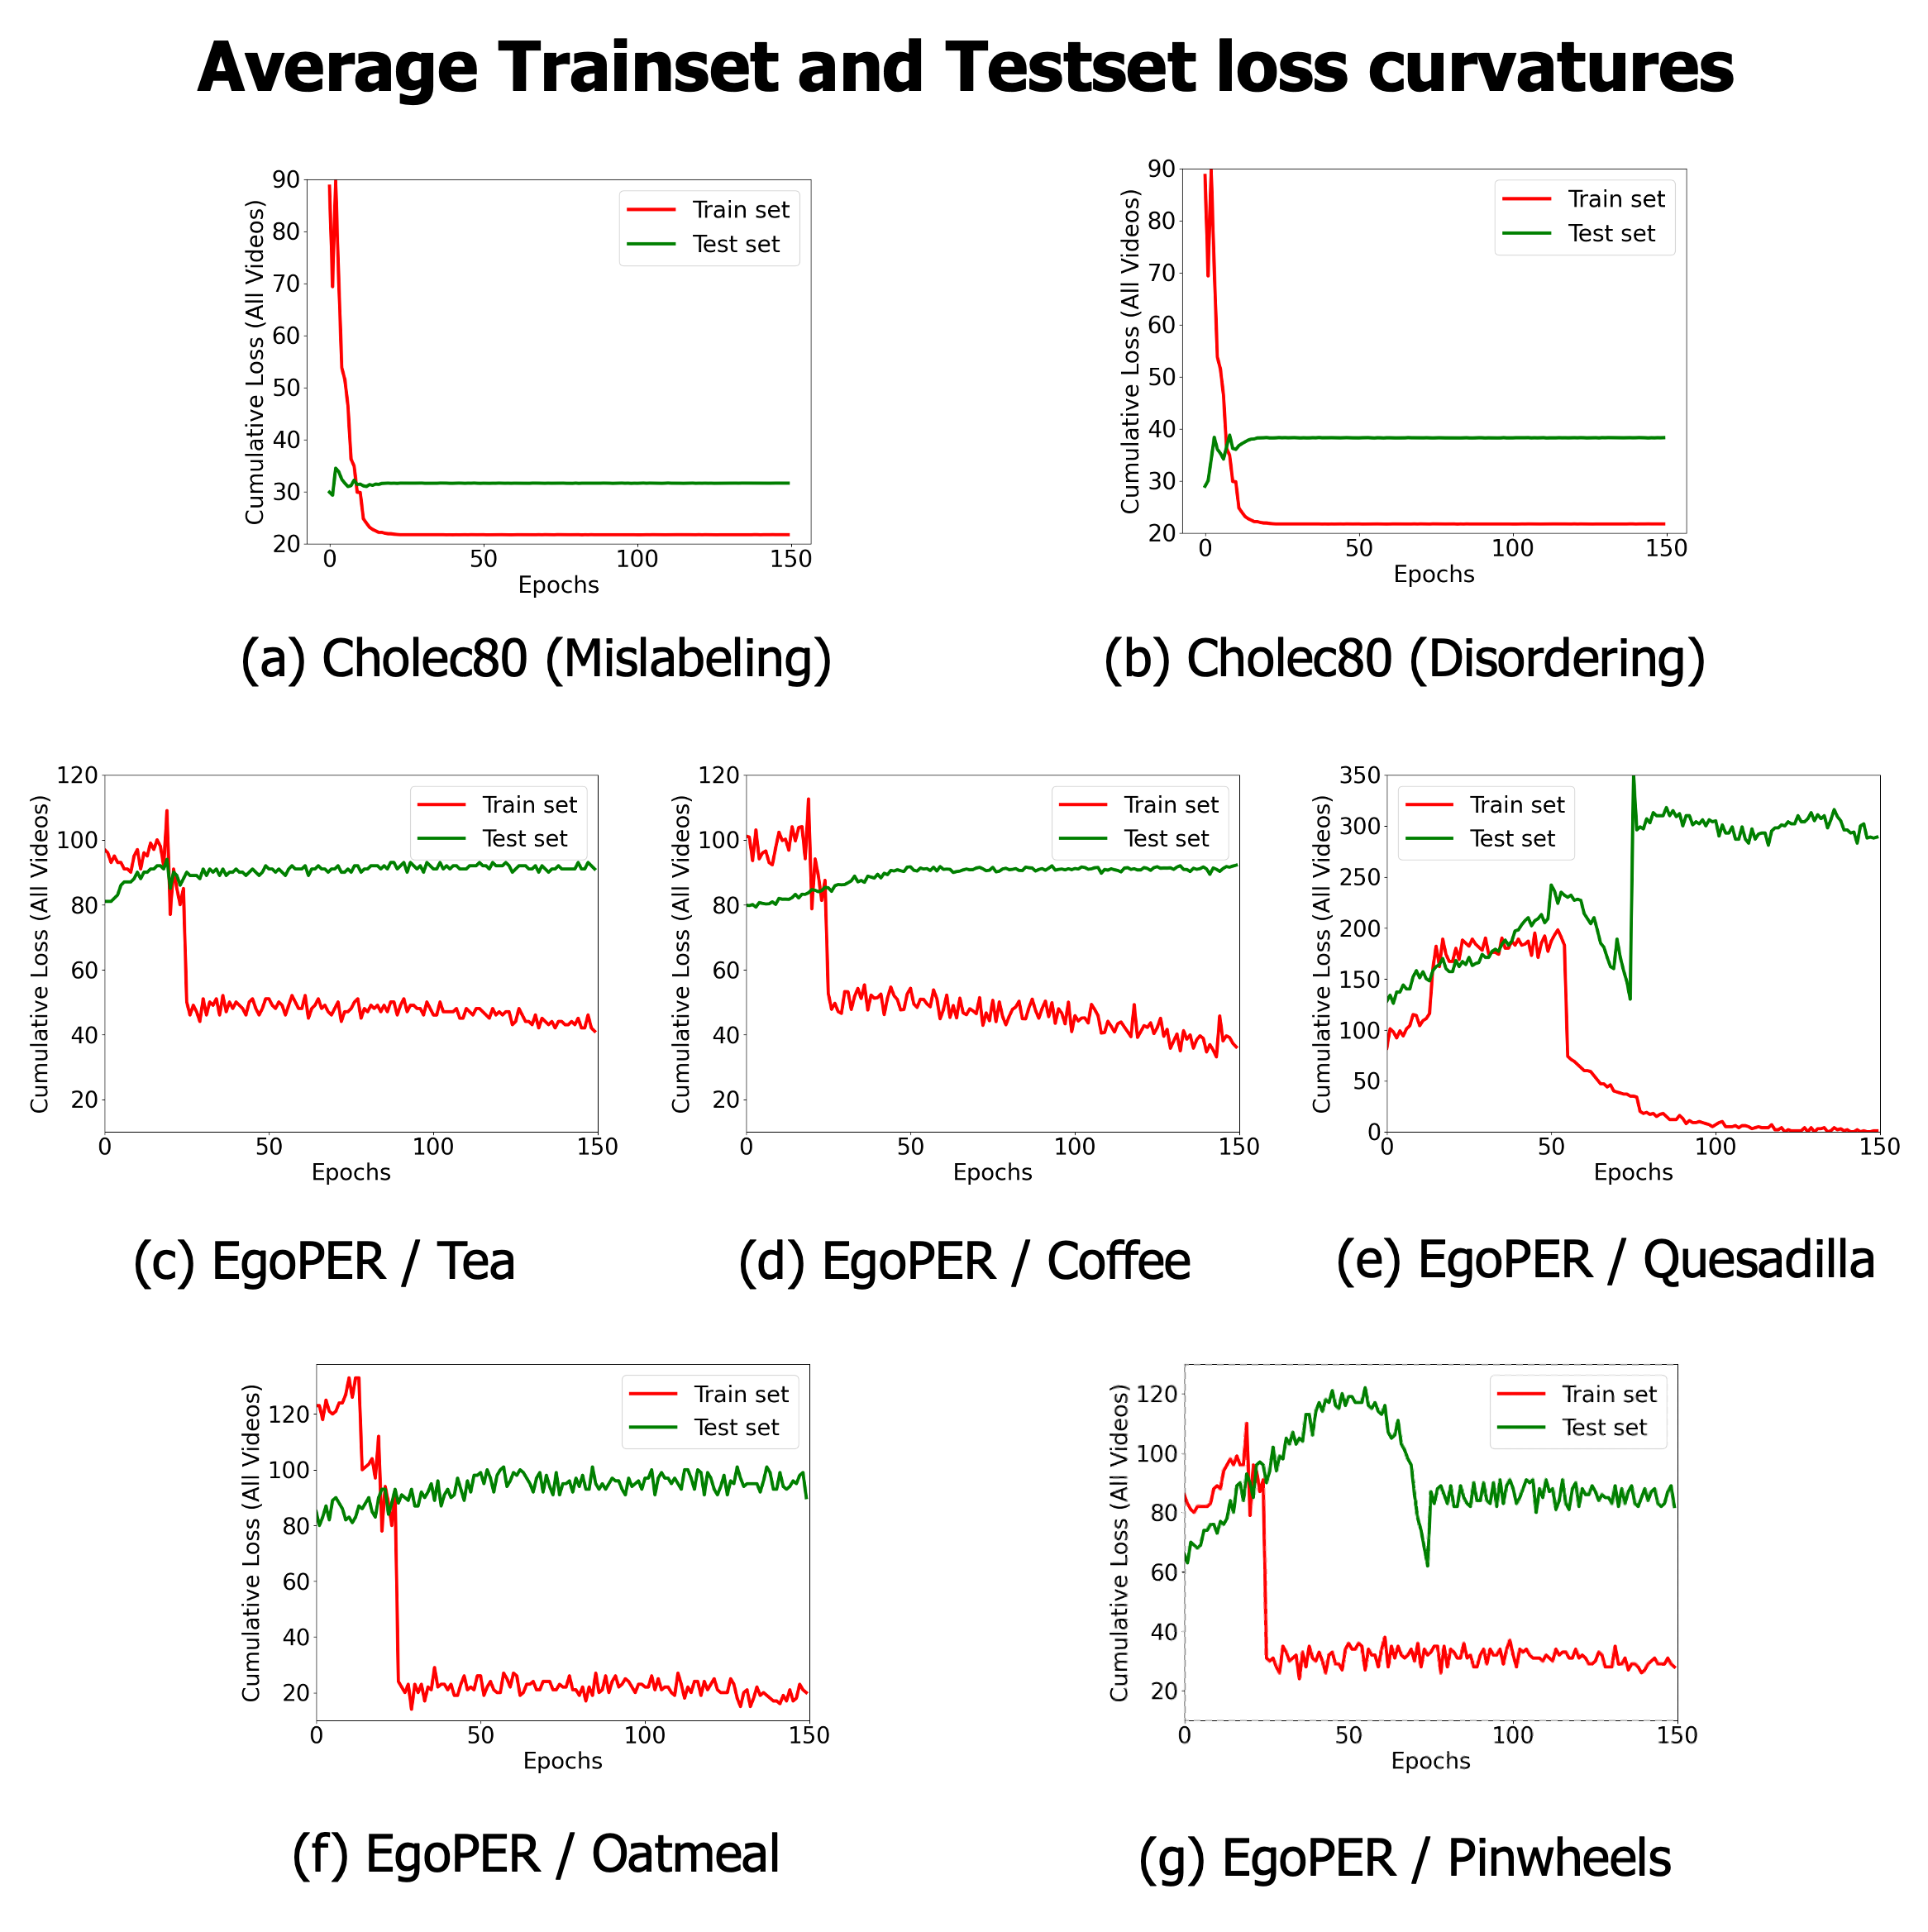
\includegraphics[width=\linewidth]{Figures/Appendix_avg_loss.png}
\caption{Average Loss trajectory across training epochs, visualized via curvature estimates on both Cholec80 and EgoPER datasets. The plots compare the average loss dynamics for the full train set and the test set. The consistently higher curvature observed in test samples highlights the persistent prediction difficulty for these frames, validating CSL as a reliable indicator of annotation defects.}
\label{fig:avg_loss}
\end{figure*}

\noindent
To further validate the proposed CSL-based framework, we analyze the curvature of loss trajectories computed from checkpoints saved at each training epoch. Figure~\ref{fig:avg_loss} illustrates the average loss dynamics for training and test samples on both Cholec80 and EgoPER.
Across datasets, correctly labeled training samples rapidly converge to low-loss regions, resulting in flatter trajectories with reduced curvature. In contrast, test samples and high-CSL examples maintain elevated loss and higher curvature throughout training. This behavior suggests persistent prediction instability and reinforces the observation that annotation defects are characterized not only by high loss magnitude but also by irregular loss evolution over time, reinforcing the utility of CSL for identifying hard-to-learn or anomalous data segments.


\section{Qualitative Visualization of CSL Dynamics Across Frame Types}
\begin{figure*}[ht]
\renewcommand{\thefigure}{A2}
    \centering
    \includegraphics[width=0.98\linewidth]{Figures/Appendix_figure1.png}    
    \caption{CSL trajectory visualization for different sample types across Cholec80 and EgoPER datasets. Each triplet shows representative frames and their cumulative sample loss (CSL) over time. Easy samples (left) show rapid loss convergence, hard samples (middle) exhibit fluctuating but bounded loss, while mislabeled samples (right) maintain high loss throughout the epochs, often exceeding a dataset-specific threshold $\tau$.}
    \label{fig:csl_maps1}
\end{figure*}

Figure~\ref{fig:csl_maps1} presents qualitative CSL trajectories for representative frames categorized as \textit{easy}, \textit{hard}, and \textit{mislabeled} across both Cholec80 and EgoPER datasets. Easy samples (green) demonstrate rapid loss reduction early in training, reflecting strong agreement between visual evidence and annotation. Hard samples (purple) show more variability but eventually converge, indicating partial ambiguity that the model resolves over time.
In contrast, mislabeled or temporally inconsistent frames (red) exhibit persistently high CSL values across checkpoints, often exceeding the threshold $\tau$. These distinct loss signatures highlight CSL's ability as a discriminative signal to separate clean, ambiguous, and corrupted annotations using loss dynamics alone.

\section{Qualitative Comparison of Annotation Defect Predictions}
\begin{figure*}[ht]
\renewcommand{\thefigure}{A3}
    \centering
    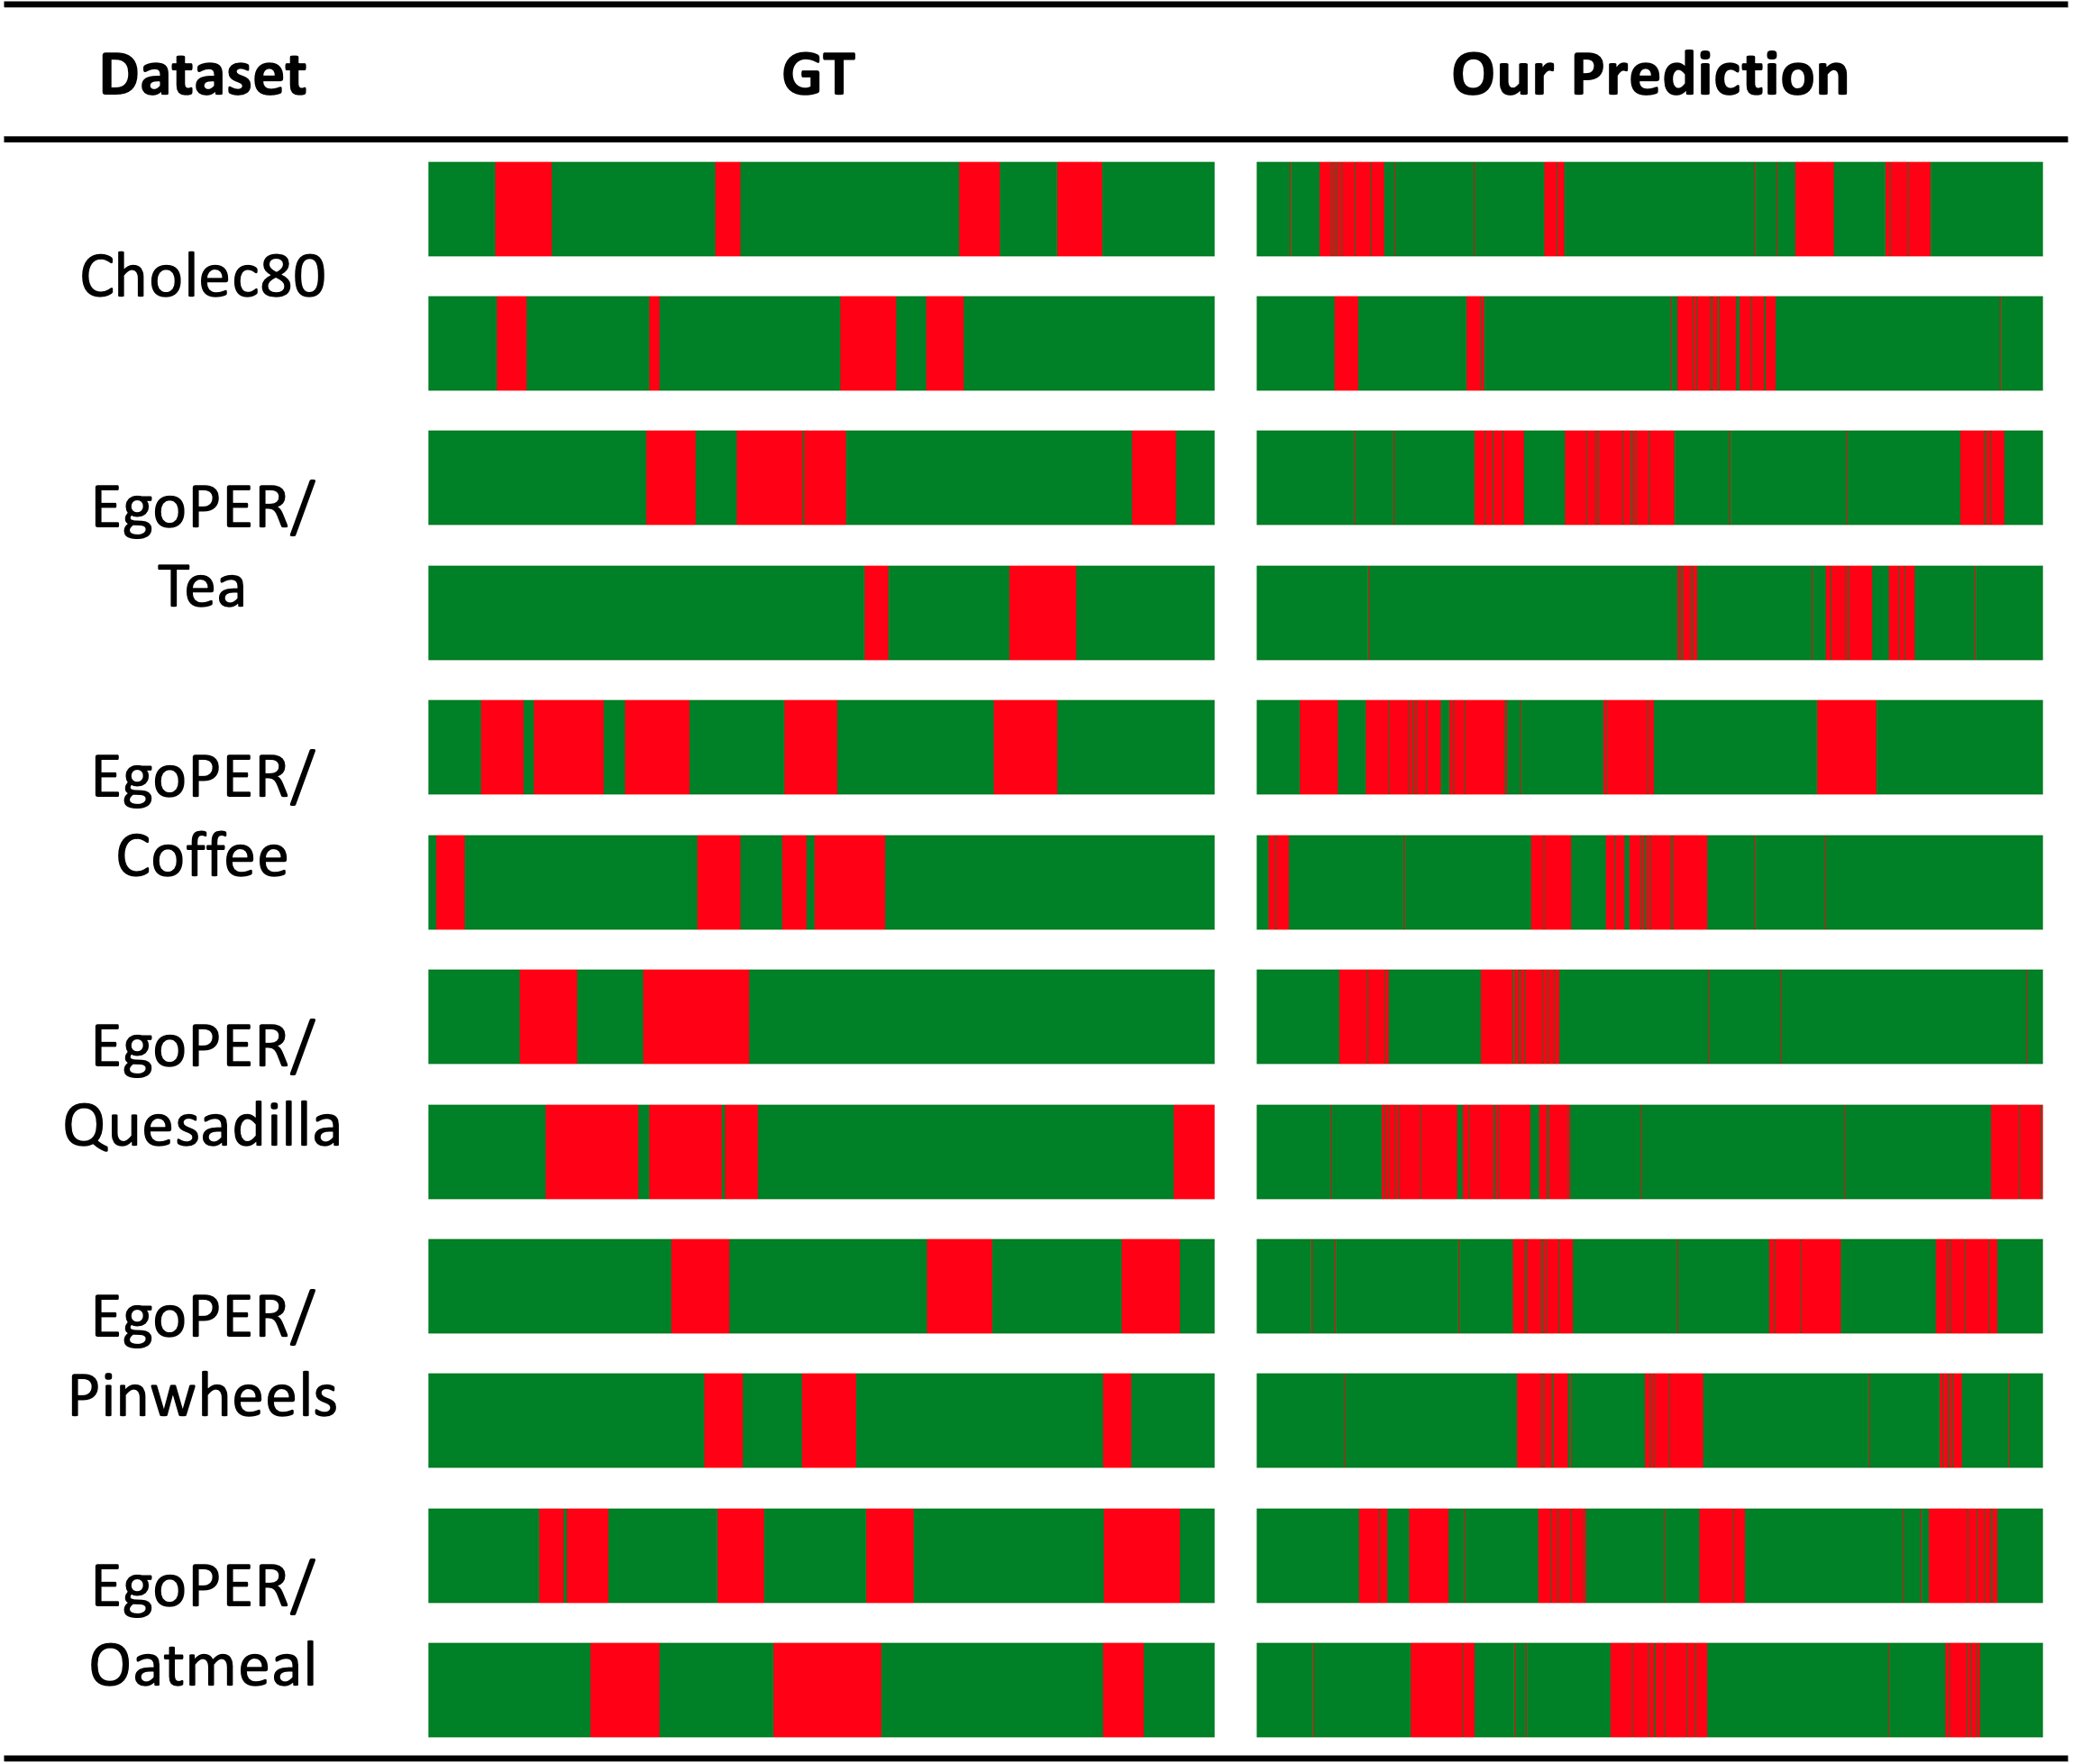
\includegraphics[width=0.98\linewidth]{Figures/Appendix_figure2.png}
    \caption{Qualitative comparison of annotation error predictions. Each horizontal bar represents a full video sequence from either Cholec80 or EgoPER. Green regions indicate correctly labeled segments, while red denotes mislabeled or disordered annotations. For each sample, we compare the ground truth annotation defects (left column) with the predictions made by our framework (right column). The results illustrate high agreement across datasets and reveal the model's ability to localize annotation defects with fine temporal granularity.}
    \label{fig:qualitative_barplot_comparison}
\end{figure*}

Figure~\ref{fig:qualitative_barplot_comparison} compares ground-truth annotation defects with predicted annotation errors across representative sequences from Cholec80 (surgical) and EgoPER (egocentric procedural) datasets. Each video is visualized as a temporal bar, where green regions correspond to correctly annotated frames and red regions denote mislabeled or disordered segments. The left column in each pair displays the ground-truth error locations, while the right column depicts the regions flagged by our CSL-based framework. 
The close alignment between predicted and ground-truth error regions demonstrates the framework's ability to localize annotation defects with fine temporal resolution. Notably, the method accurately identifies both extended mislabeling intervals and brief disordering transitions, highlighting its robustness across different error types and dataset domains.
This qualitative analysis complements our quantitative results and further demonstrates the robustness and generalizability of our framework across diverse video domains.

\section{Heatmap Visualization of Annotation Error Patterns}
\begin{figure*}[ht]
\renewcommand{\thefigure}{A4}
    \centering
    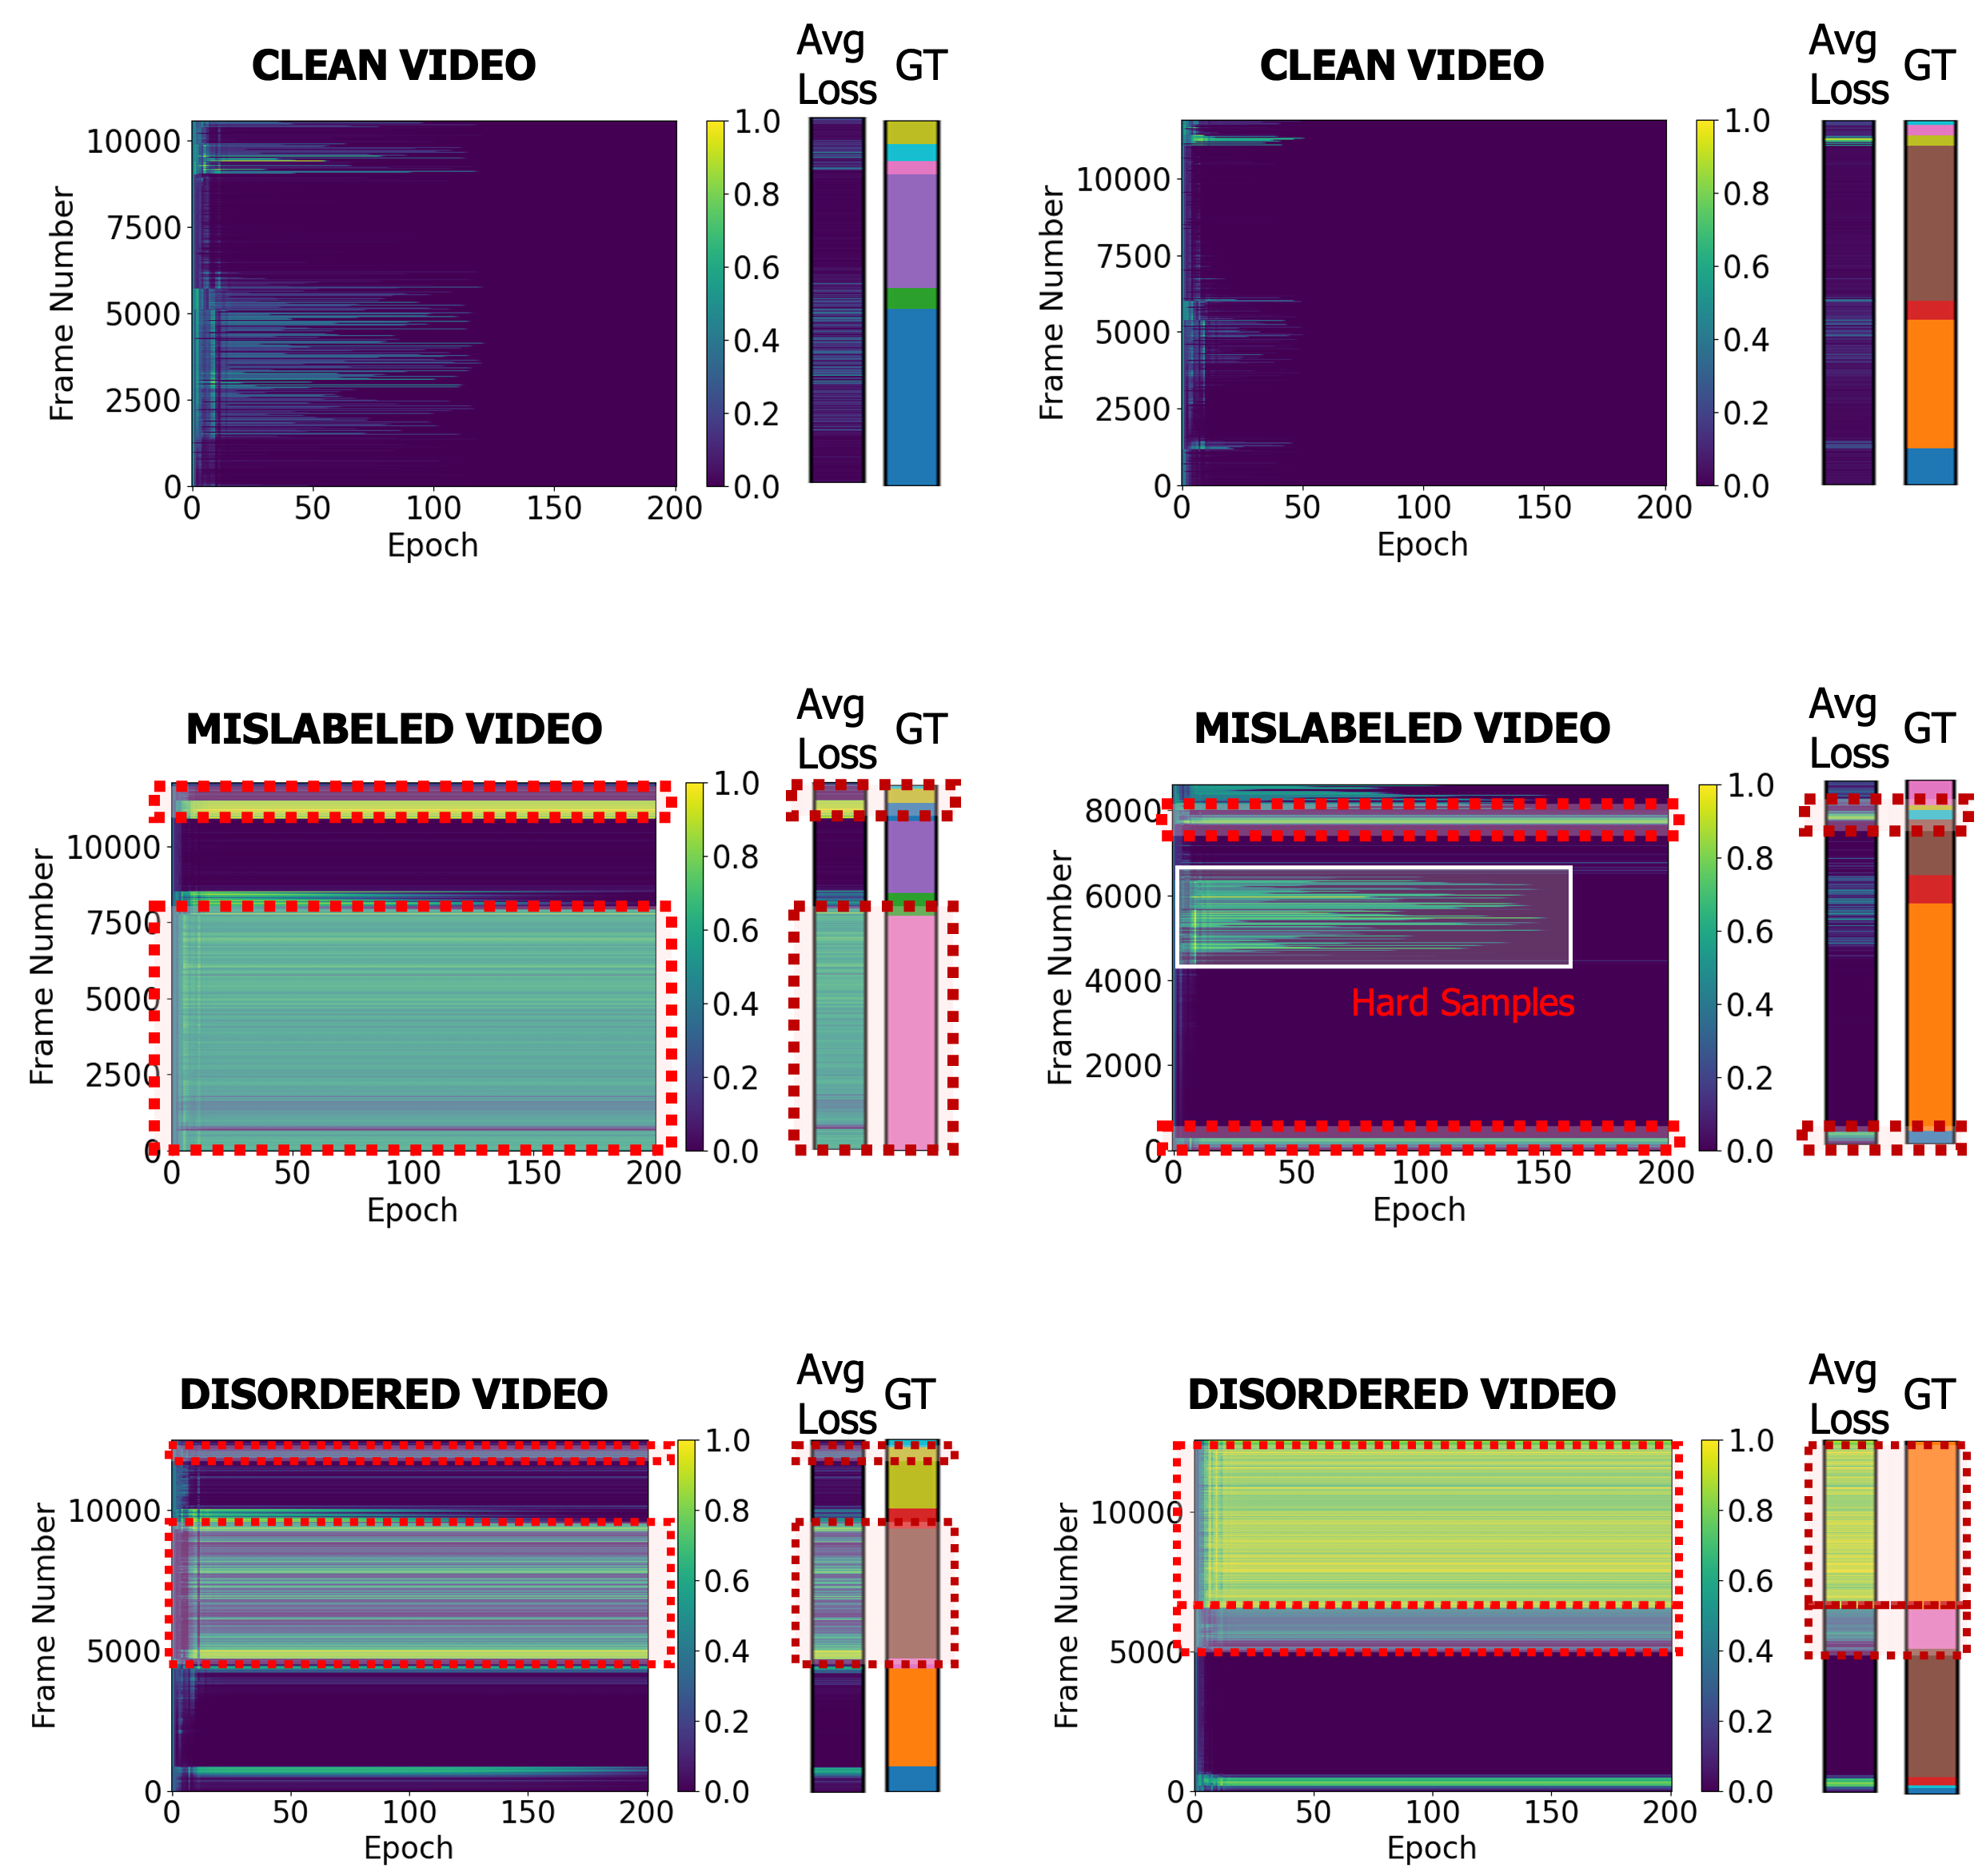
\includegraphics[width=\linewidth]{Figures/Appendix_figure3.png}
    \caption{Visualization of Sample Loss dynamics across model checkpoints. \textbf{Top Row}: Correctly labeled videos show low and uniform sample loss, indicating smooth convergence. \textbf{Middle Row}: Mislabeled segments result in globally elevated sample loss across frames, revealing persistent confusion throughout the segment. \textbf{Bottom Row}: Temporally disordered sequences exhibit sharp loss spikes around transition points, highlighting the model's sensitivity to temporal misalignment. Red dashed boxes mark high-sample loss regions caused by annotation errors.}
    \label{fig:csl_maps_ab}
\end{figure*}


Figure~\ref{fig:csl_maps_ab} visualizes CSL heatmaps for different annotation scenarios in the Cholec80 dataset. Clean sequences display consistently low loss across all checkpoints, indicating stable learning and correct supervision.
Mislabeled segments produce broad regions of elevated CSL loss, reflecting persistent disagreement between annotations and visual content. In contrast, temporally disordered sequences generate sharp, localized loss spikes around phase transitions, capturing the model's sensitivity to violations in temporal structure. 

These heatmaps visually confirm that different forms of annotation noise produce distinct loss dynamics, which can be effectively captured through CSL analysis. The red bounding boxes outline regions of significant deviation, underscoring the diagnostic capacity of our framework. Overall, these distinct patterns confirm that CSL captures both semantic and temporal annotation defects and provides an interpretable diagnostic signal for dataset auditing. 
%%%%%%%%%%%%%%%%%%%%%%%%%%%%%%%%%%%%%%%%%%%%%%%%%%%%%%%%%%%%%%%%%%%%%%%%%%%%%%%
%%%%%%%%%%%%%%%%%%%%%%%%%%%%%%%%%%%%%%%%%%%%%%%%%%%%%%%%%%%%%%%%%%%%%%%%%%%%%%%

\end{document}

% This document was modified from the file originally made available by
% Pat Langley and Andrea Danyluk for ICML-2K. This version was created
% by Iain Murray in 2018, and modified by Alexandre Bouchard in
% 2019 and 2021 and by Csaba Szepesvari, Gang Niu and Sivan Sabato in 2022.
% Modified again in 2023 and 2024 by Sivan Sabato and Jonathan Scarlett.
% Previous contributors include Dan Roy, Lise Getoor and Tobias
% Scheffer, which was slightly modified from the 2010 version by
% Thorsten Joachims & Johannes Fuernkranz, slightly modified from the
% 2009 version by Kiri Wagstaff and Sam Roweis's 2008 version, which is
% slightly modified from Prasad Tadepalli's 2007 version which is a
% lightly changed version of the previous year's version by Andrew
% Moore, which was in turn edited from those of Kristian Kersting and
% Codrina Lauth. Alex Smola contributed to the algorithmic style files.
